\documentclass[a4paper,12pt]{report}
\usepackage[slovak,english]{babel}
\usepackage[T1,IL2]{fontenc}             
\usepackage[utf8]{inputenc}    
\usepackage{amsmath}
\usepackage{amssymb,amsfonts,amscd}
\usepackage{array,hhline}
\usepackage{makeidx}
\usepackage{fancyhdr}
\usepackage{graphicx}
\usepackage{listings}
\usepackage{eurosym}
\usepackage{url,mathptmx} 
\usepackage[pdftex,unicode,bookmarks=false]{hyperref}
\usepackage{comment}
\renewcommand{\baselinestretch}{1.5} 
\addtolength{\oddsidemargin}{-.5cm}
\addtolength{\evensidemargin}{-2.9cm}   
\addtolength{\topmargin}{0cm}
\addtolength{\textheight}{0pt}
\addtolength{\textwidth}{2.cm}
\addtolength{\textheight}{2.cm}
\newlength{\verbcorr}
\setlength{\verbcorr}{0ex}
\usepackage{acronym}
%pre nastavenie formatovania kodu TODO vylepsit
\lstset{%
	language={Java},
	breaklines=true,
	breakindent=0pt,
	tabsize=2,
	showstringspaces=true
}


\usepackage{lmodern}%INE pismo
%\usepackage{type1ec}
\usepackage{float}%H pri tabulkach
%\usepackage{pdfpages}

\begin{document}


\selectlanguage{slovak}
\pagestyle{empty}
\pagenumbering{arabic}



\hypersetup{pageanchor=false} 

\begin{titlepage}
\phantom.

\bigskip

\begin{center}
{\sc\LARGE Žilinská Univerzita v Žiline}
\medskip

{\sc\Large Fakulta riadenia a informatiky}

\vfill\vfill\vfill\vfill

{\sc\LARGE Bakalárska práca}

\medskip

{\large Študijný odbor: {\bf Informatika}}
\end{center}


\vfill\vfill\vfill\vfill


\phantom.\hfill

\begin{center}
{\large\bf Oľga Chovancová}

\medskip

{\large\bf Vizualizácia dát získaných pomocou SCADA systémov s využitím HTML 5 štandartov}

\medskip

Vedúci: {\bf Ing. Juraj Veverka}\\
Tútor	\textbf{Ing. Patrik Hrkút, PhD.}
\medskip
 
\hfill
Reg.č. 5/2014
\hfill
Máj 2015
\hfill\phantom.
\end{center}

\hspace{1.7cm}\phantom.

\vspace{2.9cm}

\phantom.
\end{titlepage}
%%%%%%%%%%%%%%%%%%%%%%%%%%%%%%%%%%%%%%%%%%%%%%%%%%%%%%%%%%%%%%%%%%%%%%%%%%%%%%%%%%%%%%%%%%%%%%%%%%%%%%%%%%%%%%%%%%%%%%%%%%%%%%%%%%%%%%%%%%%%%%%%%%%%%%%%%%%%%%%%%%%%%%%%%%%%%%%%%%%%%%%%%%%%%%%%%%%%%%%%%%%%%%%%%%%%%%%%%%%%%%%%%%%%%%%%%%%%%%%%%%%%%%%%%%%%%%%%%%

%%%%%%%%%%%%%%%%%%%%%%%%%%%%%%%%%%%%%%%%%%%%%%%%%%%%%%%%%%%%%%%%%%%%%%%
\newpage

\centerline{\bf Prehlásenie}

\vspace{2em}

\noindent
Prehlasujem, že som túto prácu napísala samostatne a že som uviedola
všetky použité pramene a literatúru, z~ktorých som čerpala. 

\vspace{2em}

\noindent
V~Žiline, dňa DD.MM.2015
\hfill
Oľga Chovancová





%--------------------------------------------------------------------------------------
%%% slovensky abstrakt

\begin{abstract}

\noindent
{\sc Chovancová Oľga:} {\em Vizualizácia dát získaných pomocou SCADA systémov s využitím HTML 5 štandartov}
[Bakalárska práca] 

\noindent
Žilinská Univerzita v~Žiline,  
Fakulta riadenia a informatiky,  
Katedra softvérových technológií.

\noindent  
Vedúci: Ing. Juraj Veverka 
 
\noindent  
Stupeň odbornej kvalifikácie:
Inžinier v študijnom odbore Telekomunikačné siete, na Elektrotechnickej fakulte na Žilinskej univerzite v Žiline. 


\noindent
Tútor	Ing. Patrik Hrkút, PhD.

\bigskip

Obsahom práce je vzorová sada grafických komponentov na vizualizáciu technologických procesov s využitím HTML 5 štandardov. Jedná sa o grafické komponenty, ktoré nie sú bežne dostupné na tvorbu interaktívnych webových aplikácii ako napríklad vizualizácie mechanických súčasti hydraulických systémov, technologických liniek, silových a výkonových častí automatizačných sústav. Návrh interface, pomocou, ktorého budú tieto komponenty komunikovať so serverovou časťou SCADA systému. Cieľová platforma pre výslednú webovú aplikáciu bude kompatibilná s rodinou štandardov HTML 5 pre každý webový prehľadávač. 
\end{abstract}


%--------------------------------------------------------------------------------------
%%% anglicky abstrakt


\selectlanguage{english}
\begin{abstract}

\noindent
{\sc Chovancová Oľga:} {\em Data visualization acquired by SCADA systems using HTML5 standarts}
[Bacalar thesis] 

\noindent
University of Žilina,  
Faculty of Management Science and Informatics, 
Department of TODO.
 
\noindent
Tutor:  Ing. Juraj Veverka. 
 
\noindent
Qualification level:
Engineer in field University of Zilina, Faculty of Telecommunication, Fixed networks.
Solution Design Architect %- member of team who develops system D2000. 

\noindent
 TODO

\bigskip

The main idea of this ... TODO

\end{abstract}
\selectlanguage{slovak}
	

	

%--------------------------------------------------------------------------------------
%%% slovensky abstrakt

\begin{abstract}

\noindent
{\sc Chovancová Oľga:} {\em Vizualizácia dát získaných pomocou SCADA systémov s využitím HTML 5 štandartov}
[Bakalárska práca] 

\noindent
Žilinská Univerzita v~Žiline,  
Fakulta riadenia a informatiky,  
Katedra softvérových technológií.

\noindent  
Vedúci: Ing. Juraj Veverka 
 
\noindent
Tútor	Ing. Patrik Hrkút, PhD.

\noindent  
Stupeň odbornej kvalifikácie:
študentka na Fakulte riadenia a informatiky, odbor Informatika
%Inžinier v študijnom odbore Telekomunikačné siete, na Elektrotechnickej fakulte na Žilinskej univerzite v Žiline. 


\bigskip

Obsahom práce je vzorová sada grafických komponentov na vizualizáciu technologických procesov s využitím HTML 5 štandardov. Jedná sa o grafické komponenty, ktoré nie sú bežne dostupné na tvorbu interaktívnych webových aplikácii ako napríklad vizualizácie mechanických súčasti hydraulických systémov, technologických liniek, silových a výkonových častí automatizačných sústav. Návrh interface, pomocou, ktorého budú tieto komponenty komunikovať so serverovou časťou SCADA systému. Cieľová platforma pre výslednú webovú aplikáciu bude kompatibilná s rodinou štandardov HTML 5 pre každý webový prehliadač. 
\end{abstract}


%--------------------------------------------------------------------------------------
%%% anglicky abstrakt


\selectlanguage{english}
\begin{abstract}

\noindent
{\sc Chovancová Oľga:} {\em Data visualization acquired by SCADA systems using HTML5 standarts}
[Bacalar thesis] 

\noindent
University of Žilina,  
Faculty of Management Science and Informatics, 
Department of TODO.
 
\noindent
Tutor:  Ing. Juraj Veverka.
Tutor:  Ing. Patrik Hrkut, PhD.
 
\noindent
Qualification level:

%
%Engineer in field University of Zilina, Faculty of Telecommunication, Fixed networks.
%Solution Design Architect %- member of team who develops system D2000. 

\noindent
 TODO

\bigskip

The main idea of this ... TODO

\end{abstract}
\selectlanguage{slovak}
	

\pagestyle{empty}
\pagenumbering{arabic} 
\pagestyle{plain}	%F
\setcounter{page}{6} %F



{\setlength{\parskip}{1pt plus 1pt}

\markboth{}{}



\tableofcontents

\newpage
%
\vspace{0pt plus 2cm}
%
\listoffigures
%
\vspace{0pt plus 2cm}
%
\listoftables
}

\markboth{}{}

\clearpage



%%%%%%%%%%%%%%%%%% obsah
% table of contents

	
%\pagestyle{plain}
%\pagestyle{myheadings}

%{\setlength{\parskip}{1pt plus 1pt}
%\markboth{}{}
%\pagenumbering{arabic}
%\markboth{}{}

\clearpage
	



%\thispagestyle{empty}

%\pagestyle{plain}

%\clearpage




%\markboth{}{}

\clearpage

\setcounter{page}{11} %F

\chapter*{Úvod}
\addcontentsline{toc}{chapter}{Úvod}

Téma práce je vizualizácia dát získaných pomocou SCADA systémov. Cieľ práce je nájsť postup tvorby a vizualizácie grafických komponentov. Produktom bakalárskej práce je grafický komponent na vizualizáciu technologických procesov s využitím HTML 5 štandardov. 
V práci je popisaný detailný postup vizualizácie prečerpávaciej stanice. Bol navrhnutý jednoduchý interface, pomocou ktorého komponenty komunikujú so serverovou časťou SCADA systému. 

Návrh  interface, pomocou ktorého budú tieto komponenty komunikovať so serverovou časťou SCADA systému. 

V súčasnosti je v IPESOFT s.r.o. software, ktorý dokáže vizualizovať dáta z technológii pomocou "hrubých klientov",  čo sú natívne (.exe) Windows aplikácie a je technológia,  ktorá dokáže rovnaké dáta zobrazovať na webe. 

Aktuálna webová prezentácia takýchto dát nespĺňa súčasne štandardy pre moderné webové aplikácie a preto bolo potrebné nájsť nový spôsob vizualizácie na webe, ktorá bude v budúcnosti použiteľná na rôznych platformách, nielen na PC. 


Výsledná webová aplikácia je kompatibilná s štandardmi HTML 5. Riešenie využíva výhradne open-source knižnice s licenciami typu MIT, GNU GPL, BSD, Apache 2. Zdrojové kódy práce sú udržiavané v Git repository, dostupné na:  \url{https://github.com/chovancova/project} 

%Cieľová platforma pre výslednú webovú aplikáciu bude každý webový prehliadač kompatibilný s rodinou štandardov HTML 5. Riešenie bude využívať výhradne open-source knižnice s licenciami typu MIT, GNU GPL, BSD. Zdrojové kódy práce budú udržiavané v Git repository.

%Predbežný postup práce:
%
%\begin{enumerate}
%\item  Analýza požiadaviek, prieskum možnosti využitia \acs{WYSIWYG}\par editorov na tvorbu grafických komponent s možnosťou exportu do formátov \acs{SVG}, \acs{JSON}, \acs{XML}, alebo JavaScript.
%\item Výber vhodných open-source knižníc na tvorbu grafických komponent kompatibilných s HTML 5.
%\item Návrh \acs{REST} \acs{API} na prepojenie grafických komponent so \acs{SCADA} serverom.
%\item  Analýza možnosti automatického mapovania API grafických prvkov pomocou metadát na existujúce API dostupné pre SCADA server D2000.
%\item  Implementácia vzorovej sady grafických komponent.
%\item  Analýza výkonnosti a výkonnostné obmedzenia.
%\end{enumerate}


Postup práce: 
\begin{enumerate}
\item  Analýza požiadaviek, prieskum možnosti využitia \acs{WYSIWYG}\par editorov na tvorbu grafických komponent s možnosťou exportu do formátov \acs{SVG}, \acs{JSON}, \acs{XML}, alebo JavaScript.
\item Výber vhodných open-source knižníc na tvorbu grafických komponent kompatibilných s HTML 5.

\item Popis postupu vizualizácie grafického komponentu 
\item  Implementácia vzorovej sady grafických komponent.
\item Návrh \acs{REST} \acs{API} na prepojenie grafických komponent so \acs{SCADA} serverom.
\item  Analýza možnosti automatického mapovania API grafických prvkov pomocou metadát na existujúce API dostupné pre SCADA server D2000.

\item  Analýza výkonnosti a výkonnostné obmedzenia.
\end{enumerate}




%pridat / sucastna situacia 
%a ciel prace
%metodika vypracovani






	
% !TeX root = ../main.tex
% !TeX spellcheck = sk_SK
% !TeX encoding = UTF-8
\chapter{Základné pojmy}
V kapitole sú popísané základné pojmy. 

\section{Systémy \acs{SCADA} / HMI}

Vizualizačné systémy sú stystémy realizajúce vizualizáciu procesov. Supervisory Control and Data Acquisition / Human Machine Interface - je Supervízorové riadenie a zber údajov / Rozhranie človek stroj. 
Prenáša informáciu od stroja k ľuďom, čo umožňuje riadenie, monitorovanie a zaznamenávanie systému cez interfejs ako obrázok, klávesnicu, ethernet, touchscree, softvér atď. 


\section{\acs{HTML}5 štandard}

\ac{W3C} vydalo štandard \acs{HTML}5 dňa 28. októbra 2014. 
HTML5 je podporovaný vo všetkých moderných webových prehliadačoch. 
Na obrázku \ref{fig:obrazokHTML} je HTML5 \acs{API} a súvisiace taxonómia technológií a ich status. 

\begin{center}
	\begin{figure}[H]
\centering
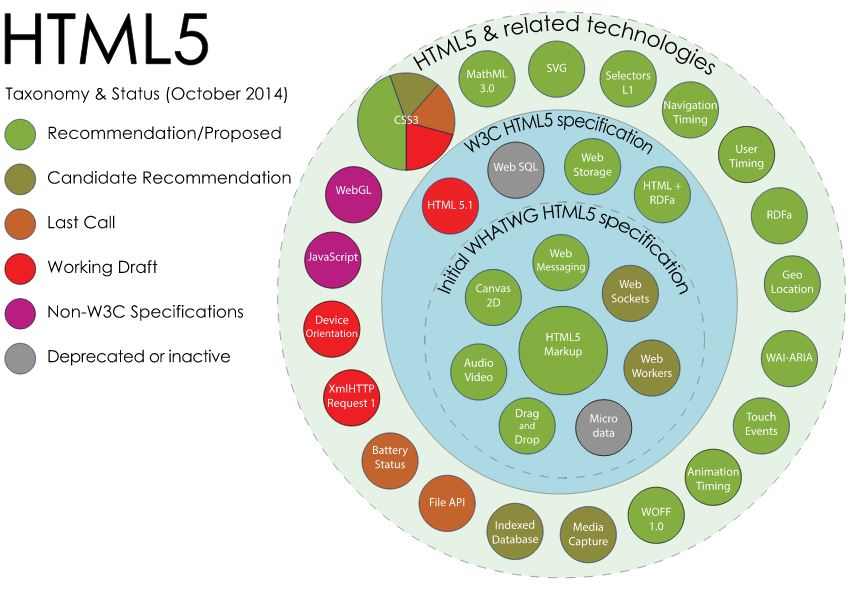
\includegraphics[width=0.7\linewidth]{obrazky/obrazokHTML}
\caption{HTML 5 API}
\label{fig:obrazokHTML}
\end{figure}
\end{center}

HTML5 Graphics definuje dva spôsoby vykreslenia využívajúc: 
\begin{itemize}
	\item $<$canvas$>$ - JavaScript
	\item $<$svg$>$ - SVG
\end{itemize}


\section{Čo je SVG?}
\ac{SVG} je štandardný formát pre vektorovú grafiku. Vektorová grafika je definovaná cez body, priamky, mnohouholníky, elipsy, krivky, alebo iné geometrické tvary.  

\acs{SVG} je jazyk na opísanie dvojrozmernej grafiky v   \ac*{XML}. Vďaka tomu, umožňuje reprezentáciu grafických informácii v kompaktnom a prenositeľnom tvare.

 SVG povoľuje tieto tri typy grafických objektov: vektorové grafické tvary, obrázky a text. 
Grafické objekty môžu byť zoskupené, štylizované, zmenené, a kombinované do predošlých vrstiev objektov. 

SVG obrázky môžu byť dynamické a interaktívne.

Prispôsobiteľnosť SVG umožňuje zmeniť veľkosť grafického komponentu bez straty kvality vzhľadu. Čo umožňuje zobraziť responzívne na viacerých možných zariadení. 
SVG sa bude zobrazovať rovnako na rôznych platformách. Je kompatibilná s štandardmi \acs{HTML}5, ktoré navrhla \ac*{W3C}. 


 \subsection{Podpora v webovom prehliadači}
 Súčasné prehliadače plne podporujú $<$svg$>$ elementy.  
  Čísla v tabuľke \ref{svgpreh} špecifikujú prvé verzie webových prehliadačov, ktoré sú schopné zobraziť $<$svg$>$ element.\cite{w3svg}
  
\begin{table}[H]
\begin{center}
		\begin{tabular}{|c|c|c|c|c|c|}
		\hline \textbf{Element} & \textbf{Chrome} & \textbf{Internet} \textbf{Explorer}  & \textbf{Firefox}  & \textbf{Safari} & \textbf{Opera}  \\ 
		\hline $<svg>$ & 4.0& 9.0 & 3.0 & 3.2  &   10.1 \\ 
		\hline 
	\end{tabular} 
\end{center}
	
	\caption{Podpora HTML $<svg>$ elementu v webových prehliadačoch}
	\label{svgpreh}
\end{table}
 
 \begin{figure}[H]
\centering
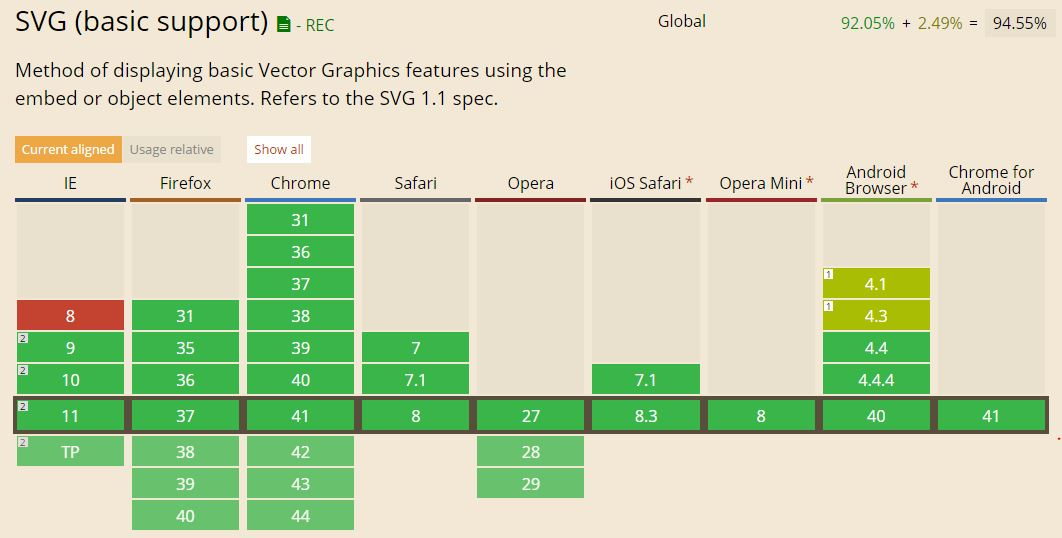
\includegraphics[width=0.7\linewidth]{obrazky/podpora}
\caption{Podpora SVG vo webových prehliadačoch}
\label{fig:podpora}
\end{figure}
% http://caniuse.com/#feat=svg
 
 \subsection{Rozdiely medzi SVG a Canvas}
 %\url{http://www.petrpexa.cz/diplomky/trantyr.pdf} strana 52

SVG patrí do vektorovej grafiky a Canvas zase do raster bitmap grafiky. 
 SVG je jazyk na opísanie dvojrozmernej grafiky v XML.  Canvas kreslí dvojrozmernú grafiku za behu programu cez JavaScript.  SVG je XML založený, čo znamená, že každý element je dostupný cez SVG DOM.   JavaScript umožňuje ovládanie udalostí elementov. V SVG je každý tvar zapamätaný ako objekt.  V prípade zmeny $<$svg$>$ elementu sa automaticky prekreslí.  
 
 
 Canvas je prekresľovaný pixel za pixelom. Bitmapová grafika je zložitejšia pre dynamické prekresľovanie, a má menšie pamäťové nároky a je rýchlejšie. 

Zariadenia ako moderné smartfóny majú veľmi vysokú hustotu pixelov. Niektoré potĺáčajú 300 \ac{PPI} s tým, že sa spoliehajú na obmedzenosť ľudských očí rozoznávať jemné detaily. Pixel nemá v reálnom živote equivalent vo veľkosti až pokým je na obrazovke s fixovaným rozmerom a rozlíšením. Text s veľkosťou 16 pixelov bude veľmi malý pre oko. Pre tento dôvod zariadenia jednoducho nezobrazujú 1 CSS pixelovú jednotku na 1 pixel zariadenia. Namiesto toho zdvoja svoju veľkosť.  
%http://www.smashingmagazine.com/2012/01/16/resolution-independence-with-svg/

%SVG and relative sizes, we have solved the three big issues highlighted above. A scalable graphic can be rasterized on demand to perfectly suit any device resolution and any zoom level. By using relative sizes, we can continue implementing a responsive design, minimizing as much as possible the need for the user to zoom. We’re also respecting the browser’s default font size, and enabling our design to adapt accordingly.


 Tabuľka \ref{canvas:SVG} zobrazuje niekoľko dôležitých odlišností medzi Canvas a SVG. 
% The table below shows some important differences between Canvas and SVG:

 \begin{table}[H]
 \centering
 \begin{tabular}{|l|p{7.5cm} |}
 	\hline \textbf{Canvas} & \textbf{SVG} \\
 	 	\hline Závislé na rozlíšení a \acs{DPI} & Nezávislé na rozlíšení a DPI \\ 
 	\hline Nepodporuje dynamické zmeny & Podporuje dynamické zmeny \\ 
 	\hline Obmedzené možnosti na vykresľovanie  & Vhodné pre aplikácie s veľkými plochami na vykresľovanie \\ 
 	\hline & Väčší výpočtový výkon pri komplexnom obrázku \\ 
 	\hline Vhodné pre grafické-intenzívne hry & Nevhodné pre dynamické hry \\ 
 	\hline 
 \end{tabular} 

 \caption{Porovnanie Canvas a SVG}
 \label{canvas:SVG}
 
\end{table}
 
 
% \section{\acs*{SVG} v HTML dokumente}
%
%SVG môže byť zobrazená buď ako inline v HTML dokumente, alebo ako vloženým samostatného .SVG súboru. 
%V tabuľke \ref{vytvorenie:SVG} sú vymenované HTML tagy na zobrazenie SVG. 
%
%
%
%\begin{table}[hp]
%	\begin{center}
%		\begin{tabular}{|l|l|}
%			\hline \textbf{Technika} & \textbf{Popis} \\ 
%			\hline $<$embed$>$ tag & Načíta vytvorený SVG súbor.  \\ 
%			\hline $<$object$>$ tag & Nepovoľuje skriptovanie.  \\ 
%			\hline $<$iframe$>$ tag & Zobrazí SVG v rámci  \\ 
%			\hline Inline & Vytvorí Svg súbor \\ 
%			\hline
%		\end{tabular} 
%	\end{center}
%	\caption{Spôsoby vytvorenia SVG v HTML dokumente}
%	\label{vytvorenie:SVG}
%\end{table}
%
%\subsection{Príklady načítania SVG v HTML dokumente}
%
%	\subsubsection{Image}
%	\begin{lstlisting}
%<img src="stanica2.svg" width = "50" height= "50" />
%	\end{lstlisting}
%	
%	\subsubsection{Embed}
%	\begin{lstlisting}
%<embed src="stanica2.svg" width = "50" height= "50" />
%	\end{lstlisting}
%	
%	
%\subsubsection{Object}
%
%	\begin{lstlisting}
%<object type="image/svg+xml" data="stanica2.svg"
%	width="50" height="50"></object>
%	\end{lstlisting}
%	
%	
%\subsubsection{	Iframe}
%
%	\begin{lstlisting}
%<iframe src="stanica2.svg" width = "50" height= "50"><</iframe>
%	\end{lstlisting}







%\subsection{Príklad použitia SVG v HTML dokumente s inline SVG}
%
%HTML kód: 
%
%\begin{lstlisting}
%<!DOCTYPE html>
%<html>
%<head lang="sk">
%	<meta charset="UTF-8">
%	<title>Bakalarska praca</title>
%</head> <body>
%	<svg width="100" height="100">
%		<circle cx="50" cy="50" r="40" stroke="black" stroke-width="2" fill="silver" />
%	</svg>	
%</body>
%</html>
%
%\end{lstlisting}
%
%SVG obrázok začína s $<$svg$>$ elementom. Atribúty elementu $<$svg$>$ sú width a height. Definujú šírku a výšku SVG obrázka. Element $<$circle$>$ je použitý na nakreslenie kruhu.
%
% Atribúty cx, cy definujú x, y súradnice od centra kruhu. Ak je cx, cy vynechané, tak center kruhu je nastavený na $($0, 0$)$. Atribút r  definuje polomer kruhu. Atribúty stroke a stroke-width určujú to ako bude vyzerať obrys útvaru. Kruh má nastavený 2px čierny okraj. 
%Atribút fill vyplní vnútro kruhu. V príklade je vyplnený sivou farbou. Tag, ktorý uzavrie SVG obrázok je $<$$/$svg$>$. Keďže SVG je validné XML, tak všetky elementy musia byť správne zatvorené. \cite{inline} Vykreslí na HTML webovú stránku útvar, ktorý je na obrázku \ref{jednoduchyKruh}.
%
%\begin{figure}[hp]
%	\begin{center}
%		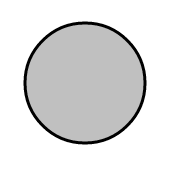
\includegraphics  {obrazky/jednoduchyKruh.png}
%		\caption{Vykreslenie SVG na HTML stránke}
%		\label{jednoduchyKruh}
%	\end{center}
%\end{figure}


%\section{SVG tvary} 
%
%\acs*{SVG} má preddefinované tvary elementov:
%\begin{itemize}
%	\item Obdĺžník $<$rect$>$
%	\item Kruh $<$circle$>$
%	\item Elipsa $<$ellipse$>$
%	\item Čiara $<$line$>$
%	\item Polyline $<$polyline$>$
%	\item Mnohouholník $<$polygon$>$
%	\item Path $<$path$>$	
%\end{itemize}
%
%Spoločné vlastnosti pre kruh, elipsu, a čiaru sú r, x, y, cx, cy, rx, ry. Teda polomer, pravá a ľavá pozícia,x a y súradnice od stredu, a horizontálny a vertikálny polomer. 
%
%\subsection{Element Path} 
%
%TODO NIECO NAPISAT K TOMU
%
%\begin{center}
%	\begin{table}
%		\begin{center}
%			\begin{tabular}{|c|l|c|}
%				\hline \textbf{Príkaz} & \textbf{Názov} & \textbf{Parametre} \\
%				\hline M & moveto & (x y)+ \\ 
%				\hline Z & closepath & (none) \\ 
%				\hline L & lineto & (x y)+ \\ 
%				\hline H & horizonal lineto & x+ \\ 
%				\hline V & vertical lineto & y+ \\ 
%				\hline C & curveto & (x1 y1 x2 y2 x y)+ \\ 
%				\hline S & smooth curveto & (x2 y2 x y)+ \\ 
%				\hline Q & quadratic Bézier curveto & (x1 y1 x y)+ \\ 
%				\hline T & smooth quadratic Bézier curveto & (x y)+ \\ 
%				\hline 
%			\end{tabular} 
%		\end{center}
%		\caption{Niekoľko príkazov na tvorbu Path elementu}
%		\label{prikazyPath}
%	\end{table}
%\end{center}

%https://msdn.microsoft.com/en-us/hh552482.aspx

	
\chapter{Postup vytvorenia komponentov}

UML diagram... 

Spôsob vytvorenia grafických komponentov je nasledovný. Najprv používateľ vytvorí SVG súbor, následne ho načíta, a vytvorí funkcie v JavaScripte na ovládanie atribútov SVG elementu. 
Alternatívna možnosť je vytvoriť SVG elementy prostredníctvom JavaScriptovej knižnice a nenačítavať súbor. 


Postup načítania SVG súboru v HTML dokumente


\begin{figure}
\centering
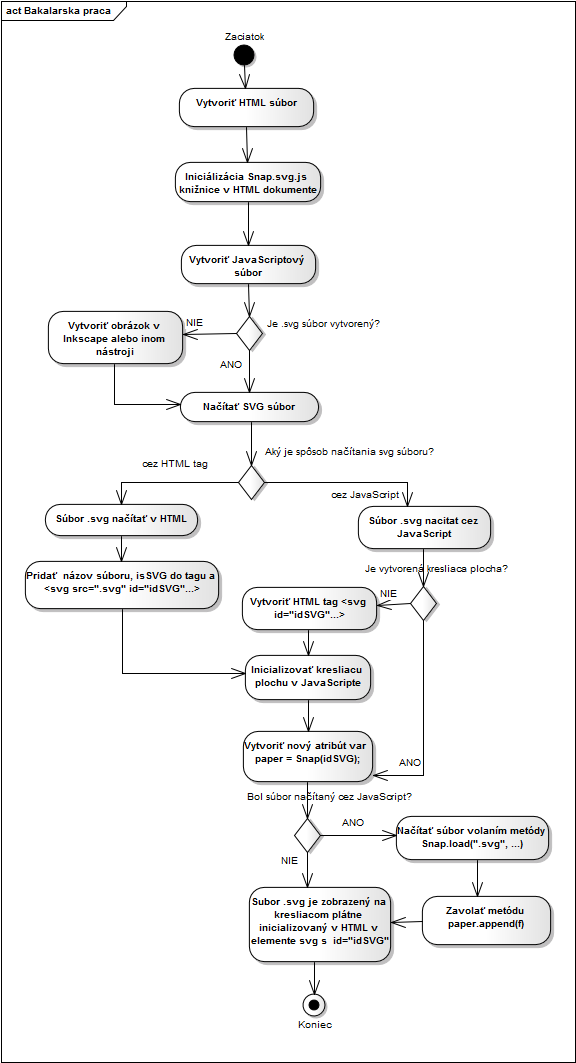
\includegraphics[width=0.75\linewidth]{uml/aktivityInicializacie}
\caption{Postup načítania SVG súboru v HTML dokumente}
\label{fig:aktivity1}
\end{figure}




\section{Použitie SVG v HTML dokumente}

SVG sa dá použiť a vytvoriť viacerými spôsobmi:
\begin{itemize}
	\item priamo v HTML dokumente - inline, 
	\item načítanie z oddeleného SVG súboru,
	\item načítanie pomocou JavaScriptovej knižnice.
\end{itemize}


 \subsection{Vytvorenenie SVG }
 
 \subsubsection{Cez program WYSWING}
 
 \subsubsection{načítanie JavaScriptovú knižnicu}

Postup (načítanie súboru v tele JavaScriptovej metóde): 
\begin{enumerate}
	\item Načítať knižnicu Snap.svg.js do HTML súboru. 
	\item Pridať atribút onPageLoad(); do definicie body.
	\item Pridať HTML tag $<$svg$>$ do tela HTML a nastaviť v ňom požadovanú veľkosť cez viewBox.
	\item Vytvoriť JavaScriptový súbor, alebo tag $<$script$>$, ktorý bude obsahovať funkcie. 
	\item Vytvorenie funkcie na načítanie Snap API, a .SVG súboru. 
	\item V tele funkcie inicializácia Snap Canvasu. To znamená, kde konkrétne v HTML stránke sa zobrazí.
	\begin{itemize}
		\item s = Snap() - najbližšie voľné miesto
		\item s = Snap(šírka, výška) 
		\item s = Snap(HTMLtag) - id tagu $<$svg$>$, ktoré sa pridalo v bode č. 3
	\end{itemize}
	\item Načítanie .SVG súboru cez funkciu Snap.load(), s parametrami: názov súboru a funkcie s parametrom f. 
	\item Zobrazenie súboru cez príkaz s.append(f);, ekvivalenté zápisy: s.appendAll(f);, s.add(f);. 
	\item V HTML stránke sa zobrazí daný .SVG súbor. 
	
	
\end{enumerate}

Postup ovládania SVG elementu:

\begin{enumerate}
	\item Vytvorenie novej funkcie. 
	\begin{itemize}
		\item anonymná funkcia 
		\item pomenovaná funkcia
		\item objekt, v ktorom bude zadefinovaná funkcia. 
	\end{itemize}
	\item Nová premenná var, ktorá obsahuje id SVG elementu, ktorý sa ide ovládať. (Na zistenie id SVG vid Postup krokov na zistenie id.)
	\item Vytvorenie funkcie cez ktorú sa bude pristupovať k API Snap knižnice. 
	\item s.select(id SVG)
	\item V tejto chvíli je možné volať funkcie z Snap API príkazom: funkcia().funkciaAPISnap.. 
	\begin{itemize}
		\item .animate() - animácia
		\item .attr() - nastavenie atribútu
		\item .add() 
		\item TODO
		\
	\end{itemize}
	
	
	
\end{enumerate}
%TODO - odkazat tuto na vsetky mozne attributy, ktore sa daju zmeniť.

	
% !TeX encoding = UTF-8
% !TeX spellcheck = sk_SK
% !TeX root = ../main.tex
%\chapter{Knižnica Snap.svg.js}





\chapter{Využitie knižnice Snap.svg.js}
%V práci cituj: \cite{Dawber} , strany sa cituju takto: \cite[p.~215]{Dawber} \\ Priklady z knihy:\url{http://raphaeljsvectorgraphics.com/}  \cite{Dawber} .
%Z tejto knihy idem pridávať do bakalárky nasledovné veci:
%Namet na zmenu: pouzit to demo, ktore mi poslal veduci na transformaciu zmeny. 


\section{Porovnanie spôsobu vykreslenia cez \acs{SVG} \acs{SMIL} a Snap}

Kreslenie vektorov je jednoduchšie cez Snap ako čisto písanie SVG. 

Príklad kreslenia obdĺžníka a animovanie šírky z 50 pixlov na 100 pixelov cez SVG SMIL:\cite[p.~9]{Dawber}
\begin{lstlisting}
<svg>
<rect x="10" y="10" width="50" height="30">
<animate attributeType="XML"
attributeName="width"
to="100"
fill="freeze"
dur="10s"  />
</rect></svg>
\end{lstlisting}

Nakreslíme obdĺžnik na súradniciach (10, 10) s šírkou 50, a výškou 30 použitím elementu $<$rect$>$. Zoskupený element $<$animate$>$ definuje animáciu zmeny šírky obdĺžnika na šírku 100 px, ktorá trvá desať sekúnd. Kde fill="freeze" je použité na zachovanie stavu obdĺžnika po ukončení animácie. Inak by bola nastavená na 50. 

Ekvivalent k animácii cez Snap API v nasledujúcom príklade:

\begin{lstlisting}
paper = Snap();
var rect = paper.rect(10, 10, 50, 30);
rect.animate({
width: 100
}, 10000);
\end{lstlisting}

Syntax metód animate a rect je výstižnejšia a lepšia na pochopenie. Snap sa tiež dobre integruje s inými knižnicami, ako napríklad jQuery. 


%%%%%%%%%%%%%%%%%%%%%%%%%%%%%%%%%%%%%%%%%%%%%%%%%%%%%%%%%%%%%%%%%%%%%%%%%%%%%%%%%%%%%%%%%%%%%%%%%%%%%%%%%%%%%%%%%%%%%%%%%%%%%%%%%%%%%%%%%%%%%%%%%%%%%%%%%%%%%%%%%%%%%%%%%%%%%%%%%%%%%%%%%%%%%%%%%%%%%%%%%%%%%%%%%%
\newpage
%Jednoduche kreslenie ,
%Interakcia ,
%Animovanie.. 
%
%Krok 0: ziskanie Snapu...


\section{Krok 1: Inicializácia plátna na kreslenie}
%viewport = výrez
Na to, aby sme boli schopní kresliť grafické komponenty, tak potrebujeme definovať miesto, kde budú vykreslené. 
%Určenie miesta, kde bude vykreslené plátno je buď viditeľné okno vo webovom prehliadači, alebo viewport. 
Viditeľná oblasť okna prehliadača, alebo viewport, definuje oblasť, v ktorej sa vykreslí komponent na plátno.
SVG špecifikácia referuje ako miesto vykreslenia seba ako viewport. 
Inak povedané viewport je akákoľvek obdĺžniková oblasť.
Okno prehliadača je referencia na viewport a kresliaca oblasť je plátno.   \cite{Dawber}


Vytvorenie plátna cez Snap konštruktor sa dá urobiť viacerými spôsobmi.

\subsection{Súradnice plátna}

TODO Na to, aby bolo plátno responzívne vo webovom prehliadači musí byť nastavené tieto dve veci: 
 \begin{itemize}
 	\item definovaný viewBox
 	\item výška a šírka plátna musí byť v relatívnych rozmeroch, najlepšie nastavená na 100\%
 \end{itemize}
 %var s = Snap("$ #s $vgout"); 
 %s.attr({ viewBox: "0 0 600 600" });
 %2. sposob pri definicii svg $ <svg id="idsvg" viewBox="0 0 600 600" weight="100\%" height="100\%"> $

Nasledujúci príkaz zadefinuje pláno s rozmermi šírka je 300 a výška 200. 
\begin{lstlisting}
var paper = Snap(300, 200);
\end{lstlisting}


Na obrázku \ref{fig:suradnice1}  je znázornená východzí súradnicový systém plátna vytvoreného cez Snap konštruktor. 
Začiatok súradnic na osi x, y je rovné nule. Bod na plátne so súradnicami x = 300, y = 200 alebo (300, 200) vo vektorovom zápisu je bod 300px vpravo od začiatku x-ovej osi a 200px dole od počiatku y-ovej osi. 

\begin{center}
	\begin{figure}[H]
		\centering
		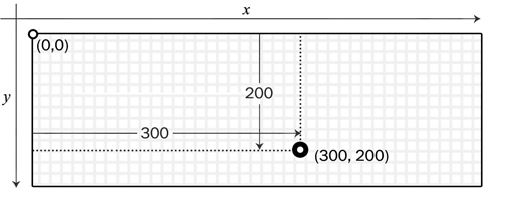
\includegraphics[width=0.5\linewidth]{obrazky/suradnice1}
		\caption{Súradnicový systém plátna s bodom (300, 200)}
		\label{fig:suradnice1}
	\end{figure}
\end{center}

\subsection{DOM element}

Dosť často je potrebné použiť existujúci DOM element ako kontajner pre plátno než viewport. Ako element môžeme použiť napríklad:
\begin{lstlisting}
<div id="mojePlatno"></div>  
\end{lstlisting}

Nasledujúcim kódom vytvorím 500px široké a 300px vysoké plátno.

\begin{lstlisting}
var paper = Snap("mojePlatno", 500, 300);
\end{lstlisting}

Keď využívam túto formu konštruktora, tak prvý element je ID elementu. Alternatívne sa dá prvý parameter DOM element napísať nasledovným spôsobom: 
\begin{lstlisting}
Snap(document.getElementById('mojePlatno'), 500, 300);
\end{lstlisting}



\subsubsection{\acs*{SVG} v HTML dokumente}

SVG môže byť zobrazená buď ako inline v HTML dokumente, alebo ako vloženým samostatného .SVG súboru. 
V tabuľke \ref{vytvorenie:SVG} sú vymenované HTML tagy na zobrazenie SVG. 


\begin{table}[H]
	\begin{center}
		\begin{tabular}{|l|l|}
			\hline \textbf{Technika} & \textbf{Popis} \\ 
			\hline
			\hline $<$embed$>$ tag & Načíta vytvorený SVG súbor.  \\ 
			\hline $<$object$>$ tag & Nepovoľuje skriptovanie.  \\ 
			\hline $<$iframe$>$ tag & Zobrazí SVG v rámci  \\ 
			\hline Inline $<$svg$>$ tag & Vytvorí Svg  \\ 
			\hline 
		\end{tabular} 
	\end{center}
	\caption{Spôsoby vytvorenia SVG v HTML dokumente}
	\label{vytvorenie:SVG}
\end{table}


%Príklady načítania SVG v HTML dokumente:
%\begin{itemize}
%\item Image 	
%\begin{lstlisting}
%<img src="stanica2.svg" width = "50" height= "50" />
%\end{lstlisting}
%\item Embed
%\begin{lstlisting}
%<embed src="stanica2.svg" width = "50" height= "50" />
%\end{lstlisting}
%\item Objekt
%\begin{lstlisting}
%<object type="image/svg+xml" data="stanica2.svg"
%width="50" height="50"></object>
%\end{lstlisting}
%\item IFrame
%\begin{lstlisting}
%<iframe src="stanica2.svg" width = "50" height= "50">
%</iframe>
%\end{lstlisting}
%\item Inline
%\begin{lstlisting}
%<svg width="100" height="100"> 
%<circle cx="50" cy="50" r="40"/> </svg>
%\end{lstlisting}
%	
%
%\end{itemize}





%%%%%%%%%%%%%%%%%%%%%%%%%%%%%%%%%%%%%%%%%%%%%%%%%%%%%%%%%%%%%%%%%%%%%%%%%%%%%%%%%%%%%%%%%%%%%%%%%%%%%%%%%%%%%%%%%%%%%%%%%%%%%%%%%%%%%%%%%%%%%%%%%%%%%%%%%%%%%%%%%%%%%%%%%%%%%%%%%%%%%%%%%%%%%%%%%%%%%%%%%%%%%%%%%%%%%%%%%
\newpage

\section{Kreslenie základných tvarov cez Snap API}

Snap API poskytuje metódy na kreslenie jednoduchých tvarov. 

\begin{table}[H]
	\begin{center}
		\begin{tabular}{|l|l|l|l|}
			\hline \textbf{Tvar} & \textbf{SVG element} & \textbf{Snap metoda} & \textbf{Atribúty} \\ 
			\hline
			\hline Obdlžnik & $<$rect$>$ & .rect() & x, y, šírka, výška, rx, ry \\ 
			\hline Kruh & $<$circle$>$ & .circle() & r, x, y, cx, cy, rx, ry \\ 
			\hline Elipsa & $<$ellipse $>$ & .ellipse() & x, y, cx, cy, rx, ry \\ 
			\hline Čiara & $<$line$>$ & .line() & x1, y1, x2, y2 \\ 
			\hline Polyline & $<$polyline$>$ & .polyline() & pole x, y suradnic bodov \\ 
			\hline Polygon & $<$polygon$>$ & .polygone() & pole x, y suradnic bodov \\ 
			\hline Path & $<$path$>$ & .path() & vid tabuľka \ref{prikazy:Path}  \\ 
			\hline 
		\end{tabular} 
		
	\end{center}
	
	\label{porovnanieSVG:Snap}
	\caption{Zoznam tvarov, ktoré podporuje SVG a Snap API, a TODO TODO POROZMYSLAT NAD NAZVOM a atributy pre definovanie tvaru}
\end{table}




Tvar, ktorý je vykreslený cez Snap API má nasledovnú syntax: 

\begin{lstlisting}
var paper = Snap(...);
var tvar = paper.NazovSnapMetody({
nazovAtributu: "hodnotaAtributu",
...
});
\end{lstlisting}

Tvar, ktorý je vykreslený priamo na HTML webovej stránke má vo vnútri elementu $<$svg$>$ definované atribúty nasledujúcim spôsobom: 

\begin{lstlisting}
<ElementTvar nazovAtributu = "hodnotaAtributu" ... />
\end{lstlisting}


\subsection{Popis atribútov tvarov}

Názvy atribútov a ich význam pre obdĺžnik, kruh, elipsu sú vyjadrené v tabuľke \ref{parametre:tvar} 

\begin{table}[H]
	\begin{center}
		\begin{tabular}{|l|l|}
			\hline \textbf{Parameter} & \textbf{Poznámka} \\ 
			\hline
			\hline x, y & súradnica x-osi, y-osi  \\ 
			
			\hline cx & x-os súradnica centra kruhu, alebo elipsy \\ 
			\hline cy & y-os súradnica centra kruhu, alebo elipsy \\ 
			\hline r & polomer kruhu, elipsy alebo okruhlých rohov na obdĺžniku \\ 
			\hline rx & horizontálny polomer elipsy \\ 
			\hline ry & vertikálny polomer elipsy \\ 
			\hline x1, y1 & začiatočné x, y súradnice \\
			\hline x2, y2 & konečné x, y súradnice \\
			
			%\hline width, height & šírka, výška\\
			\hline
		\end{tabular} 
		
	\end{center}
	\caption{Názvy atribútov a ich význam}
	\label{parametre:tvar}
\end{table}

Pre útvary polyline, polygon sú atribúty dvojice súradníc osi x, y, ktoré určujú body, ktoré sa spoja. 



\subsubsection{Path tvar}


V Snap API je to metóda Paper.path([pathString]), ktorá vytvorí $<$path$>$ element podľa daného reťazca.  Parameter pathString pozostáva reťazca skladajúceho sa z jedno písmenkových príkazov, nasledovanými bodkami a oddeľovaný argumentami a číslami. Príkazy sú uvedené v tabuľke \ref{prikazy:Path}.

Napríklad: "M10,20L30,40" - obsahuje príkazy: M s argumentami (10, 20) a L (30, 40). Rozdiel vo veľkosti písma vyjadruje to, či ide o absolútnu, alebo relatívnu cestu. Ak sú malé znaky jedná sa o relatívne, v prípade veľkých znakov absolútna cesta. 


\begin{center}
	\begin{table}[H]
		\begin{center}
			\begin{tabular}{|c|l|c|}
				\hline \textbf{Príkaz} & \textbf{Názov} & \textbf{Parametre} \\
				\hline
				\hline M & moveto & (x y)+ \\ 
				\hline Z & closepath & (none) \\ 
				\hline L & lineto & (x y)+ \\ 
				\hline H & horizonal lineto & x+ \\ 
				\hline V & vertical lineto & y+ \\ 
				\hline C & curveto & (x1 y1 x2 y2 x y)+ \\ 
				\hline S & smooth curveto & (x2 y2 x y)+ \\ 
				\hline Q & quadratic Bézier curveto & (x1 y1 x y)+ \\ 
				\hline T & smooth quadratic Bézier curveto & (x y)+ \\ 
				\hline 
			\end{tabular} 
		\end{center}
		\caption{Niekoľko príkazov na tvorbu Path elementu}
		\label{prikazy:Path}
	\end{table}
\end{center}


\section{Vykreslenie obrázku}
Snap povoľuje vloženie bitmapových obrázkov (.jpg alebo .png) na plátno. Používa metódu image z Paper objektu. Parametre metódy image sú: zdroj, x, y, šírka, výška. Príklad kódu, ktorý vkladá .jpg obrázok do plátna:
\begin{lstlisting}
var paper = Snap("mojePlatno", 300, 200);
paper.image("obrazok.jpg", 15, 15, 100, 150);
\end{lstlisting}


\section{Atribúty elementu}

Tvary, ktoré sa dajú nakresliť sa môžu vyfarbiť, orámovať alebo mnoho iných atribútov sa dá nastaviť. Keď sa vytvorí tvar, tak sa vráti Element objekt. Tento objekt má attr metódu, ktorá akceptuje key-value pár atribútov. V tomto odseku sa pozrieme na rôzne atribúty, ktoré môžu byť aplikované na naše grafické komponenty používajúc túto metódu. 

%Element.attr(...) vráti alebo nastaví dané atribúty elementu. Medzi parametre patrí buď objekt, ktorý sa skladá s páru kľúč-hodnota, alebo názvu atribútu. 

\subsection{Výplň elementu - fill }

Pozadie pre element nastavím cez metódu attr použitím fill atribútu ako parameter. Pre jednofarebné výplne je formát vyjadrený cez CSS špecifikáciu. CSS špecifikácia farieb je nasledovná: \#rrggbb alebo skrátene \#rgb , rgb(r, g, b) reťazec alebo slovne. 
Napríklad: 
\begin{lstlisting}
var kruh = paper.circle(50, 50, 40).attr("fill", "red");
\end{lstlisting}

Ďalšie spôsoby výplne elementu sú obrázkom,  gradientom, alebo vzorom. 
Pre nastavenie neprehľadnosti nastavíme atribút "fill-opacity" hodnotou čísla v rozsahu od 0-1. Element pri "fill-opacity": 1 je neprehľadný.  

\subsection{Nastavenie okraja elementu - stroke}

Elementy môžu mať niekoľko rôznych druhov okrajových atribútov. Prehľad tých najznámejších je v tabuľke \ref{parametre:styl}.\cite{styly}


\begin{table}[H]
	\begin{center}
		
		\begin{tabular}{|l|l|l|}
			\hline \textbf{Atribút pre attr() } &\textbf{CSS atribút} & \textbf{Poznámka} \\ 
			\hline 
			
			\hline stroke & stroke & farba výplne okraja \\ 
			\hline strokeWidth & stroke-width & šírka okraja v px, default je 1 \\ 
			\hline
			strokeOpacity & stroke-opacity & neprehľadnosť, 0-1 \\
			\hline strokeLinecap & stroke-linecap & ["butt", "square", "round"], tvar - okraj konca\\ 
			\hline strokeLinejoin & stroke-linejoin & ["bevel", "round", "miter"], tvar - okraj roku\\ 
			
			\hline strokeDasharray &stroke-dasharray & pole čiarok, bodiek.., napr.5,3,2\\
			
			\hline
		\end{tabular} 
	\end{center}
	\caption{Výber možných stroke atribútov}
	\label{parametre:styl}
\end{table}


\section{Zoskupovanie elementov}

Niekedy je potrebné použiť rovnaké atribúty, transformácie, alebo animácie pre viacero elementov. V Snap API je možné využiť metódu group alebo g. Group zoskupí viacero elementov do množiny. Príkazom add sa dajú pridať ďalšie prvky. V množine sa dajú meniť atribúty pre viacero prvkov naraz volaním metódy attr. 

Príklad zoskupenia elementov. Výsledné zoskupenie je zobrazené na obrázku \ref{fig:grupovanieElementov}. 

\begin{lstlisting}
var paper = Snap();
var kruh = paper.circle(50, 50, 40);
var obdlznik = paper.rect(120, 10, 80, 80);
var elipsa = paper.ellipse(270, 50, 40, 20);

var group = paper.g(kruh, obdlznik);
group.add(elipsa);

group.attr({
	fill: 'yellow',
	stroke: '#000',
	strokeWidth: 5, 
	strokeDasharray: [3, 5, 1]
});
\end{lstlisting}

\begin{figure}[H]
\centering
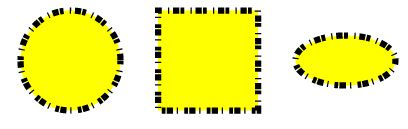
\includegraphics[width=0.7\linewidth]{obrazky/grupovanieElementov}
\caption{Príklad zoskupenia elementov a následná zmena atribútov}
\label{fig:grupovanieElementov}
\end{figure}








%
%
%\newpage
%\clearpage
%TOTO BUDE PRIKLAD KED BUDEM MAT UZ NAPISANE ATTRIBUTY NA ZMENU STYLU
%asi by bolo velmi vhodne pouzit nejake ine demo, ako ubohy kruh, teda asi teplomer, alebo mapu, ale urcite nieco ine ako kruh!!!!!!!!!!
%
%\subsubsection{PRIKLAD TVORBY KRUHU A NASTAVENIE ATRIBUTOV }
%
%Kód vytvoreného kruhu: 
%
%\begin{lstlisting}
%<svg width="100" height="100">
%<circle cx="50" cy="50" r="40" stroke="black" stroke-width="2" fill="silver" />
%</svg>	
%\end{lstlisting}
%
%SVG obrázok začína s $<$svg$>$ elementom. Atribúty elementu $<$svg$>$ sú width a height. Definujú šírku a výšku SVG obrázka. Element $<$circle$>$ je použitý na nakreslenie kruhu.
%
%
%TODO TODO TODO
%
%Atribúty stroke a stroke-width určujú to ako bude vyzerať obrys útvaru. Kruh má nastavený 2px čierny okraj. 
%Atribút fill vyplní vnútro kruhu. V príklade je vyplnený sivou farbou. Tag, ktorý uzavrie SVG obrázok je $<$$/$svg$>$. Keďže SVG je validné XML, tak všetky elementy musia byť správne zatvorené. \cite{inline}
%
%Kruh vytvorený cez Snap API má nasledovný kód:
%
%\begin{lstlisting}
%var paper = Snap(100, 100);
%var kruh = paper.circle(50, 50, 40);
%kruh.attr({
%stroke: "black", 
%strokeWidth: 2, 
%fill: "silver"
%});
%
%\end{lstlisting}
%
%
%Vykreslí sa na HTML stránku obrázok \ref{jednoduchyKruh}. Obidva spôsoby vykreslili kruh na webovej stránke úplne rovnako.  
%
%\begin{figure}[hp]
%	\begin{center}
%		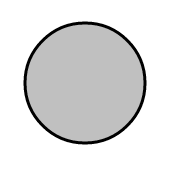
\includegraphics  {obrazky/jednoduchyKruh.png}
%		\caption{Vykreslený kruh vytvorený cez SVG, a Snap API}
%		\label{jednoduchyKruh}
%	\end{center}
%\end{figure}
%
%

%\subsection{Maskovanie - Element.mask()}
%TODO - 
%PRE DANY ELEMENT VOLAM FUNKCIU ATTR, KDE NASTAVIM VLASTNOST MASK 
%NAPR. mask: ellipse
%
%/ Now more interesting stuff
%// Let's assign this group as a mask for our big circle
%bigCircle.attr({
%	mask: discs
%});

\section{Práca s textom - Paper.text(x, y, text)}

Vykreslenie textu na plátne namiesto HTML markup s CSS štýlovaným umožňuje animovať a transformovať v rovnakým spôsobom ako iné tvary. Text vytvorení cez metódu text. Parametre metódy text sú súradnice x, y a text, ktorý sa vykreslí. Vlastnosti textu sa dajú zmeniť volaním metódy attr. V tabuľke sú atribúty, ktoré sa dajú zmeniť prostredníctvom metódy attr. 


\begin{table}[H]
	
	\begin{center}
		
		\begin{tabular}{|l|l|p{8cm}|}
			\hline \textbf{Snap atribút}  &\textbf{ CSS atribút}  & \textbf{Poznámka} \\ 
						\hline
			\hline font & font & napr. "30px Helvetica, sans-serif",\\ 
			\hline textAnchor & text-anchor & pozícia textu, napr. "middle" \\ 
			\hline fill & fill & výplň textu farbou, gradientom, vzorom \\ 
			\hline fontSize  & font-size  & veľkosť textu  \\ 
			\hline fontFamily & font-family & napr. "monospace" \\ 
			\hline fontStyle & font-style  & štýl písma, napr. kurzíva  \\ 
			\hline fontVariant  & font-variant  & napr. "small-caps"  \\ 
			\hline  fontWeight & font-weight  &  hrúbka písma,  napr. normal, bold, bolder, lighter, 100-900\\ 
			\hline 
		
		\end{tabular} 
		
		
	\end{center}
\label{tab:text}
\caption{Atribúty na zmenu vlastností elementu text}
\end{table}

Príklad zmeny farby: 
\begin{lstlisting}
var paper = Snap();
var text = paper.text(30, 100, "Namestovo");

text.attr({
	textAnchor: "middle",
	fill: "#00b", 
	fontSize: '16px', 
	fontFamily: "Veranda", 
	fontStyle: "italic", 
	fontVariant: "small-caps", 
	fontWeight: 800, 
});
\end{lstlisting}

Na obrázku \ref{fig:textPriklad} je zobrazený text, ktorý bol uvedený v príklade. 

\begin{figure}[H]
\centering
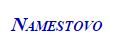
\includegraphics{obrazky/textPriklad}
\caption{Príklad na zmenu atribútov v texte.}
\label{fig:textPriklad}
\end{figure}


\newpage




\section{Transformácie - Element.transform(...)}



"t100,100r30,100,100s2,2,100,100r45s1.5"
Each letter is a command. There are four commands: t is for translate, r is for rotate, s is for scale and m is for matrix.

There are also alternative “absolute” translation, rotation and scale: T, R and S. They will not take previous transformation into account. For example, ...T100,0 will always move element 100 px horisontally, while ...t100,0 could move it vertically if there is r90 before. Just compare results of r90t100,0 and r90T100,0.

So, the example line above could be read like “translate by 100, 100; rotate 30 stupnov around 100, 100; scale twice around 100, 100; rotate 45 stupnov around centre; scale 1.5 times relative to centre”. As you can see rotate and scale commands have origin coordinates as optional parameters, the default is the centre point of the element. Matrix accepts six parameters.

Usage
\begin{lstlisting}


var el = paper.rect(10, 20, 300, 200);
// translate 100, 100, rotate 45, translate -100, 0
el.transform("t100,100r45t-100,0");
// if you want you can append or prepend transformations
el.transform("...t50,50");
el.transform("s2...");
// or even wrap
el.transform("t50,50...t-50-50");
// to reset transformation call method with empty string
el.transform("");
// to get current value call it without parameters
console.log(el.transform());
\end{lstlisting}






Keď vytváram element v Snap, tak efektívne vytváram \ac{DOM} objekt. TODO... \cite [page~51] {Dawber} 

\subsection{Suradnicovy system}

\subsection{Jednoduché transformácie}

Transformácia je realizovaná cez metódu Element.transform(), ktorá má v parametri transformačný string. Pri transformácii sa dá využiť klonovanie elementov cez metódu Element.clone(). Syntax transformačného stringu je vyjadrené z príkazov, ktoré sú v tabuľke \ref{tab:trasf}. 

\begin{table}[H]
	
	\begin{center}
		
		\begin{tabular}{|c|c|c|c|}
			\hline \textbf{Názov} & \textbf{Príkaz} & \textbf{Parameter} & \textbf{Príklad} \\ 
			\hline Preloženie & T, t & x, y & t50,100 \\ 
			\hline Rotácia& R, r & uhol, (bod rotacie x, y) & r45,0,0 \\ 
			\hline Škála & S, s & scale x, y, (scale bod x, y) & S 2,4.5,75,125 \\ 
			\hline 
		\end{tabular} 	
	\end{center}
	\label{tab:trasf}
	\caption{Syntax transformačného stringu}
	
\end{table}

Transformačný string využíva malé a veľké varianty príkazov. Variant s veľkými písmenami znamená to, že sa transformuje, bez ohľadu na predchádzajúcu transformáciu. Opačne to je pri variante s malými písmenami, ktoré berú na vedomie predošlú transformáciu.\cite[p.~52]{Dawber} 

V SVG sa vytvorí k elementu nový tag animateTransform, kde sa nastaví attributeName na transform, a typ a hodnoty sú uvedené v tabuľke \ref{tab:svgTrans}. 

\begin{table}[H]
	\begin{center}
		\begin{tabular}{|l|p{9cm}|}
			\hline \textbf{Transformation} & \textbf{Popis} \\ 
			\hline translate(x,y) & Posunie súradnicový systém na dané x, y.  \\ 
			\hline scale(xFactor, yFactor) & zmena mierky, ak je uvedená len jedna hodnota, prehliadač predpokladá, že obidve hodnoty sú rovnaké. \\ 
			\hline rotate(uhol) & Zrotuje súradnice o daný uhol. Stred rotácie je (0,0).  \\ 
			\hline rotate(uhol, centerX, centerY) & Zrotuje súradnice o daný uhol, s danými súradnicami stredu rotácie.  \\ 
			\hline skewX(uhol) &  Skosenie pozdĺž osi X.  \\ 
			\hline skewY(uhol) &  Skosenie pozdĺž osi Y.  \\ 
			\hline 
		\end{tabular} 
		
	\end{center}
	\label{tab:svgTrans}
	\caption{Typy transformácií vo vnútri SVG tagu animateTransform }
\end{table}


\subsubsection{Translation}

Element.transform("T 300 0);
todo \cite{Dawber}[p~53]

\subsubsection{Rotation}

Element.transform("t 100 0 r 180 220 100");

\subsubsection{Scaling}

Element.transform("t 100 0 s 1.2 0.5");

TODO je tam este toho dost o tych maticiach.. a


\subsection{Event handler}
tuto by som porovnala ake su predefinovane v svg,a ake su v javascripte.. 
onstart, onend, onmove, draffing, dropping, 

Transformation je dost rozsiahla.. 



\chapter{Návrh vzorovej sady grafických komponentov}

V programe Inkscape som vytvorila nasledujúcu sadu grafických komponentov. Vzorová sada grafických komponentov SCADA systémov obsahuje:
\begin{itemize}
	\item Prečerpávacia stanica - obrázok \ref{fig:pump} umožňuje meniť indikátor prítoku na červenú alebo zelenú. Je možné spustiť alebo zastaviť rotáciu motora a animovať stúpanie a klesanie hladiny v nádrži. 
	\item Prepravný pás - obrázok \ref{fig:belt} znázorňuje pohyb elementu po páse, pričom sa dá meniť pozícia elementu od 0 po 100 udaná v percentách. 
	\item Trojcestný ventil - obrázok \ref{fig:trippleValve} znázorňuje dva motory, ktoré sa dajú spustiť a zastaviť, čo je znázornené rotáciou vrtuliek. Ak je ventil zelený, je otvorený a ak je červený, tak je zatvorený a nepriepustný.   
	\item Mapa Slovenska - obrázok \ref{fig:map} umožňuje zmenu farby jednotlivých krajov, pridanie a zmeny farby textu, umožňuje pridať element na predefinovanú cestu a animovať pohyb medzi jednotlivými bodmi. 
	\item Thermometer - obrázok \ref{fig:thermometer} animuje pohyb stúpania alebo klesania teploty na určitú hodnotu. Hodnota sa zadáva v percentách. 
\end{itemize}

Vytvorila som interface metód, ktoré majú obsahovať jednotlivé grafické komponenty. Sú zobrazené v diagrame tried, ktoré sú na obrázku \ref{fig:classD}


\begin{figure}[hp]
	\centering
	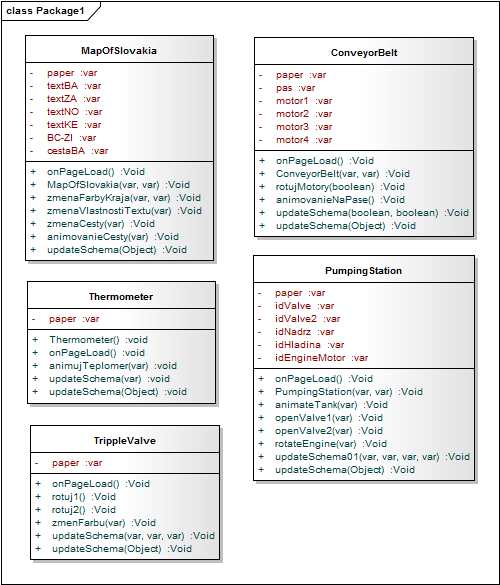
\includegraphics[width=0.9\linewidth]{uml/classDiagramTried.png}
	\caption{Diagram tried vzorovej sady grafických komponentov}
	\label{fig:classD}
\end{figure}


\begin{figure}[H]
	\centering
	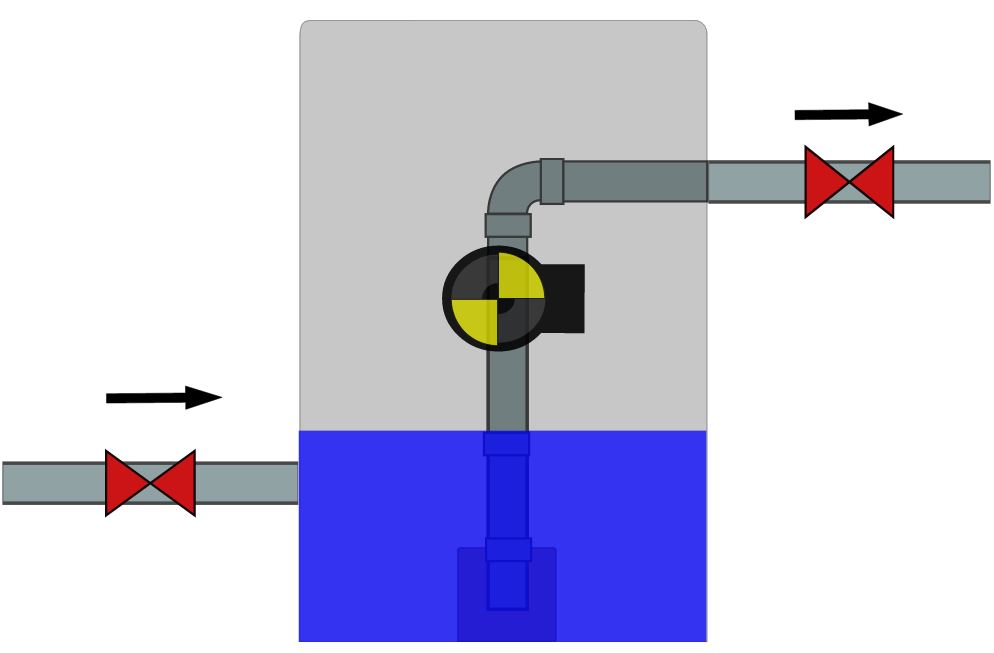
\includegraphics[width=0.7\linewidth]{obrazky/pump}
	\caption{Prečerpávacia stanica}
	\label{fig:pump}
\end{figure}
%%%%%%%%%%%%%%%%%%%%%%%%%%%%%%%%%%%
\begin{figure}[H]
	\centering
	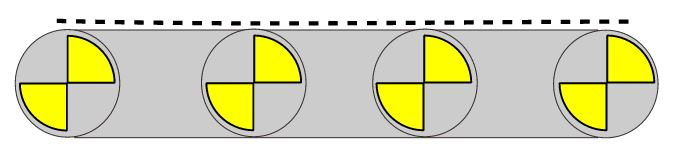
\includegraphics[width=0.7\linewidth]{obrazky/belt}
	\caption{Prepravný pás}
	\label{fig:belt}
\end{figure}
%%%%%%%%%%%%%%%%%%%%%%%%%%%%%%%%%
\begin{figure}[H]
	\centering
	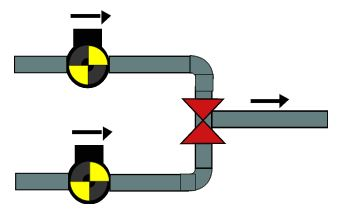
\includegraphics[width=0.7\linewidth]{obrazky/trippleValve}
	\caption{Trojcestný ventil}
	\label{fig:trippleValve}
\end{figure}
%%%%%%%%%%%%%%%%%%%%%%%%%%%%%%%%%%%%%%%%%
\begin{figure}[H]
	\centering
	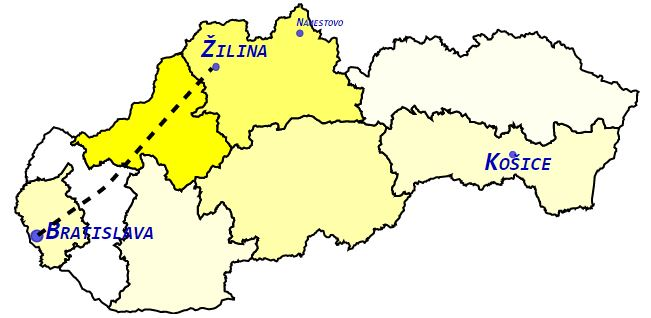
\includegraphics[width=0.7\linewidth]{obrazky/map}
	\caption{Mapa Slovenska}
	\label{fig:map}
\end{figure}
%%%%%%%%%%%%%%%%%%%%%%%%%%%%%%%%%%%%%%%%%
\begin{figure}[H]
	\centering
	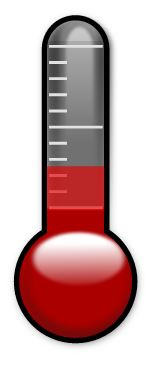
\includegraphics[width=0.2\linewidth]{obrazky/thermometer}
	\caption{Termometer}
	\label{fig:thermometer}
\end{figure}
\chapter{Integrácia grafického komponentu}

V tejto kapitole bližšie popíšem implementáciu prečerpávacej stanice. 

\section{Vytvorenie prečerpávacej stanice v Inkscape}

Nakreslenie jednotlivých častí komponentov prečerpávacej stanice v Inkscape bolo realizované pomocou ľavého bočného panela. Prečerpávacia stanica sa skladá z potrubí, indikátora úrovne hladiny vody, motora, a dvoch symbolov prítoku hladiny. Ako je možné vidieť na obrázku  \ref{picture1}.  


\begin{figure}[H]
	\begin{center}
		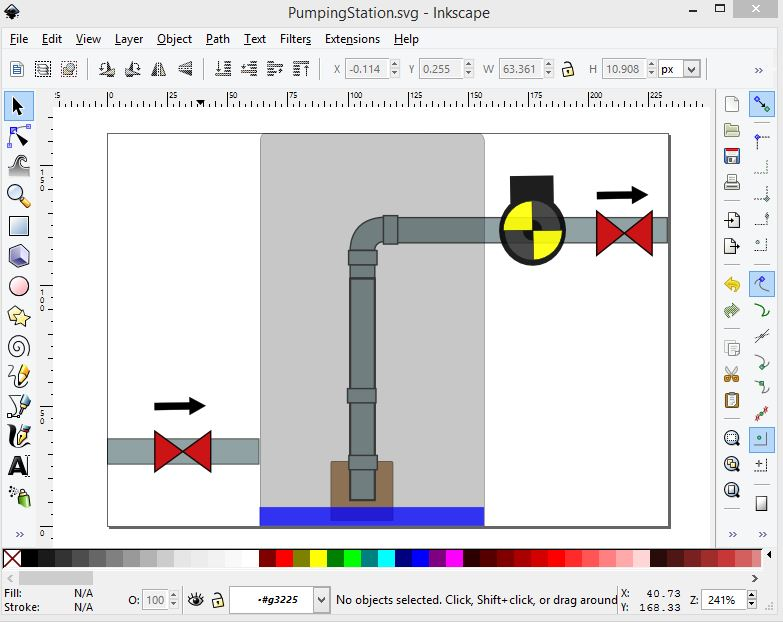
\includegraphics[width=0.6\linewidth] {obrazky/pump1.jpg}
		\caption{Grafické prostredie programu Inkscape s nakreslenou prečerpávacou stanicou}
		\label{picture1}
	\end{center}
\end{figure}


\section{Definovanie id v SVG}

Pre ovládanie JavaScriptom je nutné si pozrieť jednotlivé jedinečné identifikačné názvy. V .svg súboroch sú označované ako id. V zdrojovom kóde .svg súboru je to označené id="nazovElementu". Na ovládanie časti svg elementu v JavaScripte bude realizované cez CSS selektor, kde pristúpim k id svg cez značku \#.  Napríklad: paper.select("\#ventil"); .


\subsection{Object Properties}
Zistenie id je pomerne jednoduché v Inkscape. Klikneme pravým tlačidlom na daný komponent, ktorého id chceme vedieť, a potom na Objekt Properties.

Po kliknutí sa nám zobrazí okno s názvom Object Properties. 

\begin{figure}[H]
	\begin{center}
		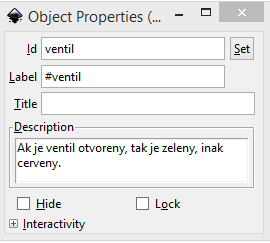
\includegraphics [width=5cm]  {obrazky/obr3.png}
		\caption{Object Properties}
		\label{picture3}
	\end{center}
\end{figure}


Z obrázka č.\ref{picture3} možno vyčítať aké je ID, predvolené sú tam napríklad desc3072. Hodnoty je možné prepísať a zmeniť stlačením tlačidla Set. Pre nás je dôležitá hodnota v kolónke id - ventil. 

V okne Object Properties je možné nastaviť script na animovanie. Po kliknutí na Interactivity sa zobrazia ďalšie kolónky, kde je možné zadať akciu, ktorá má nastať.  


\subsection{XML Editor}
Ďalší spôsob získania informácii o svg cez Inkscape je cez zabudovaný XML Editor.
Stlačením klávesovej skratky SHIFT + CTRL + X alebo v hornej lište v menu vybrať ponuku Edit a na spodku je XML Editor. Následne sa zobrazí okno, ktoré je na obrázku \ref{xmlEditor}. XML Editor umožní zistiť ID jednotlivých komponentov, ale i hodnoty atribútov. 

\begin{figure}[H]
	\begin{center}
		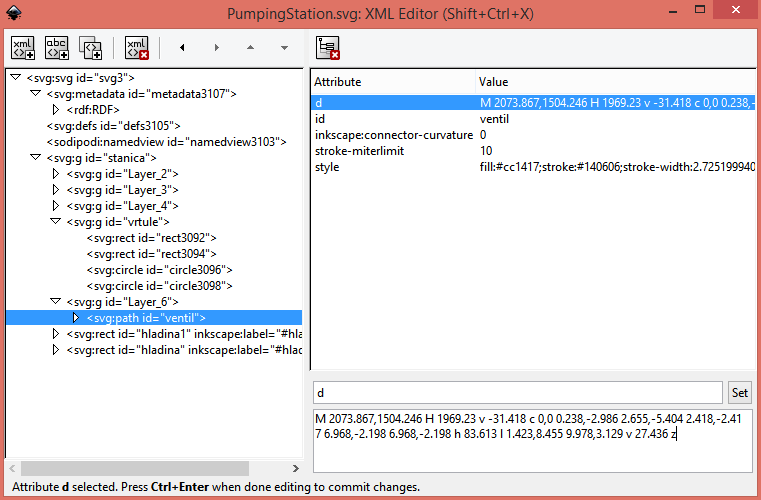
\includegraphics[width=0.6\linewidth]  {obrazky/XmlEditor2.png}
		\caption{Xml Editor v Inkscape}
		\label{xmlEditor}
	\end{center}
\end{figure}



\section{Integrácia prečerpávacej stanice pre dynamické ovládanie SVG objektu}

Súborová štruktúra prečerpávacej stanice: 
\begin{itemize}
	\item index.html 
	\item PumpingStation.js
	\item PumpingStation.svg
	\item TestPumpingStation.js
\end{itemize}

\subsection{HTML súbor}
Do HTML súboru index.html pridáme párový tag $<$svg$>$.  Na toto miesto sa neskôr vykreslí SVG načítané zo súboru cez JavaScript. Môže sa tu uviesť i celý kód SVG obrázka. V prípade, že nebude v dokumente dané, kde presne sa nachádza SVG, tag tak sa pridá na najbližšie voľné miesto. 
\subsection{Kód}
\begin{lstlisting}
<svg 
	id="svgStanica" 
	viewBox="0 0 750 600" 
	width="100%" 
	height="100%"> 
</svg>
\end{lstlisting}

\subsection{Vysvetlenie kódu}
Atribúty v tagu sú prispôsobené na to, aby sa grafický element vykreslil responzívne na obrazovku.
\begin{itemize}
\item  \textbf{id} - jedinečný identifikátor. 
\item 	\textbf{viewBox} - je virtuálne okno, ktorým sa užívateľ uvidí svg obrázok. Je atribút, ktorý povoľuje špecifikovať danú množinu grafických komponentov, aby sa zobrazili v daných súradniciach x, y a šírke, výške. Hodnoty atribútov v viewBox sú štyri čísla - min-x, min-y, width a height. 
\item 	\textbf{width} a \textbf{height} je šírka a výška. Hodnoty atribútov je možné uviesť relatívne v percentách alebo absolútne v pixloch. 
\end{itemize}

Do HTML dokumentu sa pridajú jednotlivé JavaScriptové knižnice s ktoré bude daný grafický komponent používať. 
\begin{lstlisting}[language = HTML]
<script src="../js/snap.svg-min.js"></script>
<script src="PumpingStation.js"></script>
\end{lstlisting}

Musíme sa uistiť, aby sa načítali všetky JavaScriptové knižnice, pred spustením funkcií. To zabezpečíme pridaním  onload do tagu $<$body$>$. 
\begin{lstlisting}[language = HTML]
	<body onload="onPageLoad();">
\end{lstlisting}



\section{PumpingStation.js}
V súbore PumpingStation.js sú metódy na vizualizáciu grafického komponentu. V tejto časti je popis jednotlivých funkcií. 
Interface prečerpávacej stanice: 
\begin{itemize}
	\item onPageLoad();
	\item PumpingStation(nazovFileSVG, idDOMsvgElement);
    \item openValve1(isOpenValve1);
    \item animateTank(intPercent);
    \item rotateEngine(isRotating);
    \item openValve2(isOpenValve2);
    \item updateSchema01(isOpenValve1, intPercent, isRotating, isOpenValve2);
    \item updateSchema(updateData);
\end{itemize}

\subsection{onPageLoad()}
onPageLoad() sa spustí pri načítaní tela HTML súboru index.html. Následne spustí  PumpingStation(par1,, par2). Prvý parameter je udaný svg súbor vytvorení programom Inkscape. Druhý parameter je id tagu svg, kde sa vykreslí prečerpávacia stanica.

\begin{lstlisting}
function onPageLoad() {
	PumpingStation("PumpingStation.svg", "#svgStanica" );
}
\end{lstlisting}

\subsection{PumpingStation(par1, par2)}

Parametre pre PumpingStation sú názov svg súboru, a id, ktoré sa nachádza v tagu $<$svg$>$ html súbore.

Vo vnútri PumpingStation sa nachádza inicializácia globálnych atribútov. 
\begin{lstlisting}[language = HTML]
var paper;
var idValve, idValve1 idNadrz, idHladina, idEngineMotor;

function PumpingStation(nazovFileSVG, idDOMsvgElement) {
	paper = Snap(idDOMsvgElement);
	Snap.load(nazovFileSVG, function (f) {
		idHladina = "#hladina";
		idNadrz = "#nadrz";
		idValve = "#ventil";
		idValve2 = "#ventil2";
		idEngineMotor = "#engineMotor";
		paper.append(f);
	});
}
\end{lstlisting}

Atribút paper je globálna premenná cez ktorú sa bude pristupovať k metódam JavaScriptovej knižnice Snap.svg. Jej parameter je referencia na plochu, kde bude vykreslené SVG elementy.

Vo vnútri funkcie sa volá z Snap.svg API funkcia load(). Má parametre názov súboru, a funkciu, ktorú spustí následne po načítaní. 
Vo vnútri funkcie load() sa inicializujú globálne premenné.  
Premenné obsahujú CSS selektor id získaný z programu Inkscape. Premenné budú slúžiť ako parameter pri volaní funkcie paper.select(). Pre prípadné zmeny v id, sa dané id zmení na jednom mieste a nemusí sa prepisovať všade. 

Význam premenných je nasledový: 
\begin{itemize}
	\item idHladina - indikátor prítoku hladiny vody, 
	\item idNadrz - je miesto, kde bude prichádzať prítok vody,
	\item idValve1, idValve2 - je ventil, 
	\item idEngineMotor - je symbol rotora motora.
\end{itemize}

Načítaný .svg súbor sa zobrazí volaním metódy append. 

\subsection{animateTank(percento)}
V tejto metóde je zobrazená vizualizácia prítoku hladiny do nádrže. Ako parameter slúži percento vyplnenia. 

\begin{lstlisting}[language = HTML]
function animateTank(percento){
	var height = paper.select(idNadrz).getBBox().height;
	var y = paper.select(idNadrz).getBBox().y;
	var newHeight = height * (percento/100);
	var newY = y + height - newHeight;
	
	paper.select(idHladina).animate({
	y: newY,
	height: newHeight
	}, 1000);
}
\end{lstlisting}

Animovanie je realizované cez metódu animate zo Snap.svg API. 
Význam lokálnych premenných: 
\begin{itemize}
	\item height - výška nádrže do, ktorej bude pritekať voda,  získaná volaním metódy getBBox(),
	\item y - súradnica y - navýšením, alebo znížením hladiny sa mení súradnica y, a x zostava nezmenená,
	\item newHeight - vypočítaná nová výška hladiny podľa daného percenta, 
	\item newY - je vypočítaná súradnica - osi y. 
\end{itemize}

Volaním metódy animate, sa zanimuje daný element, v tomto prípade to bude hladina nádrže. Metóda má nasledovné parametre: \begin{itemize}
	\item atribúty - v pároch udané atribúty, ktoré sa zmenia. Zmení sa iba výška a os y, ostatné atribúty zostávajú nezmenené.
	\item rýchlosť animácie udaná v milisekundách. 
\end{itemize}

 
\subsection{openValve1(isOpen)}
Indikátor prítoku hladiny do prečerpávacej stanice je ventil, ktorý mení farbu. Ak je nastavený parameter isOpen na true, tak farba ventila bude zelená, v inom prípade červená. 
Zmena farby je realizovaná volaním metódy attr zo Snap.svg API, ktorá nastavila atribút fill daného elementu na danú farbu. Farba zmeny je zapísaná termálnym operátorom. 
Pre zmenu farby v druhom elemente je zápis identický až na to, že je zmena pri volaní select - na idValve2. 
\begin{lstlisting}
function openValve1(isOpen){
	paper.select(idValve).attr({
	fill: ((isOpen === "true") ?   "green" : "red")
	});
}
\end{lstlisting}



\subsection{rotateEngine(isRotating)}
Táto metóda bude rotovať až dovtedy pokým sa nezmení parameter isPaused. Rotácia motora je zabezpečená vnorenou metódou rotateLeft. Tá sa volá v toggleRotation(), kde v má parameter element vrtuliek čerpadla. 

Popis metódy rotateLeft():
\begin{itemize}
\item animationRunning - nastavené na true, znamená to, že animácia ešte beží
\item stringT0 - je transformačný string - potrebný na rotáciu vrtuliek čerpadla. Uhol rotácie je nulový, a súradnice stredovej osi x, y sú získané volaním metódy elementu getBBox().cx a getBBox().cy. 
\item transform() - je metóda z Snap.svg knižnice, ktorá umožní nastaviť transformáciu rotácie, kde parametrom je transformančný string. 
\item if(!(isPaused)){..} - je podiemka, ktorá zaručí opakované rotovanie elementu. 
\item stringT360 - je transformačný string, ktorý zrotuje element o uhol 360 stupňov zo stredom súradnicovej osi elementu. 
\item animate() - je metóda, kde animujem transformáciu z uhlu 0 stupňov na 360 stupňov. Ako parametre sú:
\subitem - párový atribút transform s hodnotou transformačného stringu, 
\subitem - rýchlosť animácie v milisekundách - 2000 ms, 
\subitem - mina objekt, ktorý zaručí lineárny plynulý pohyb, 
\subitem - callback funkcia, ktorá sa spustí po dokončení animácie. Toto zabezpečí opakované spustenie animácie rotácie elementu. 
\item else - ak skončí animácia - tak sa nastaví animationRunning na hodnotu false. 
\end{itemize}

\subsubsection{Kód metódy} 
\begin{lstlisting}
var isPaused = true;
var animationRunning = false;
function rotateEngine(isRotating){
	isPaused = isRotating;

	function toggleRotation() {
		if (!animationRunning && isPaused) {
			isPaused = false;
			rotateLeft(paper.select(idEngineMotor));
		} else {
			isPaused = true;}
	}
	toggleRotation();

	function rotateLeft(element) {
		animationRunning = true;
		var stringT0 = "R0,"+ element.getBBox().cx 	+ ","+
		element.getBBox().cy;
		element.transform(stringT0);

	if (!(isPaused)) {
		var stringT360 = "R360,"+ element.getBBox().cx 	+ ","+
		element.getBBox().cy;
		element.animate({
		 transform: stringT360 },
		 2000, 
		 mina.linear, 
		 rotateLeft.bind(null, element));
		} else { animationRunning = false;}
	}
}
\end{lstlisting}


\section{updateSchema()}

Metóda updateSchema01 zabezpečí aktualizáciu grafického komponentu. Parametre má nasledovné: 
\begin{itemize}
\item isOpenValve - boolean hodnota, ktorá nastaví indikátor prítoku vody, v prípade true - na zelený, v opačnom na červený. 
\item intPercento - je integer hodnota v rozsahu od 0-100. Vyjadruje percentuálne naplnenie nádrže. 
\item isRotating - boolean hodnota, ktorá nastaví otáčanie motora, až pokým sa znova nezavolá. 
\item isOpenValve - boolean hodnota druhého ventila. 
	
\end{itemize}

\begin{lstlisting}
function updateSchema01(isOpenValve1, intPercent, isRotating, isOpenValve2) {
	openValve1(isOpenValve1) ;
	animateTank(intPercent);
	rotateEngine(isRotating);
	openValve2(isOpenValve2);
}
\end{lstlisting}

Dáta vyjadrené vo formáte \ac*{JSON}. Zároveň je to interfejsná metóda k grafickému komponentu Pumping Station. Toto je príklad objektu update dátami na nastavenie hladiny nádrže na 20 percent a s ventilami, a rotorom zapnutým.  
\begin{lstlisting}
var updateData = {
	"valve1": "true",
	"tank": "20",
	"engineRotation": "true",
	"valve2": "true"
};
\end{lstlisting}
Metóda updateSchema s parametrom objekt updateData, aktualizuje grafický komponent na dané hodnoty. Zároveň je  to interfejsná metóda k REST API prečerpávacej stanice. Na obrázku \ref{fig:updateSchema} je zobrazený animovaný komponent s vopred pripravenými dátami. 
\begin{lstlisting}
function updateSchema(updateData){
	updateSchema01(updateData.valve1, updateData.tank, updateData.engineRotation, updateData.valve2);
}
\end{lstlisting}


\begin{figure}[H]
\centering
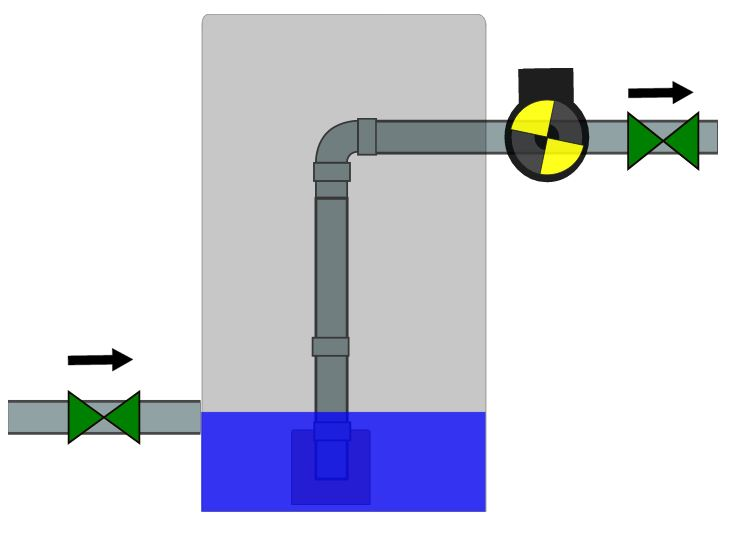
\includegraphics[width=0.7\linewidth]{obrazky/updateSchema}
\caption{Prečerpávacia stanica po vykonaní príkazu updateSchema(updateSchema);}
\label{fig:updateSchema}
\end{figure}
\chapter{REST API}

\section{REST API pre grafické komponenty}
Grafické komponenty pre vizualizáciu dát zo systému D2000 budú umiestňované na HTML stránkach použitých ako súčasť web rozhrania frameworku D2000 WebSuite.

Tento framework je založený na technológii Java Enterprise Edition a Java Server Faces.

Životný cyklus webovej stránky - načítanie stránky s technologickou schémou, pre prvé zobrazenie kompletnej schémy je potrebný plný dáta set.


Príklad REST URL:\\
\url{http://localhost:8080/scada-demo/rest/pumpingstation/gatfulldataset}


Príklad JSON dát z grafického komponentu prečerpávacia stanica: 
\begin{lstlisting}
var updateData = {
	"valve1": "false",
	"tank": "0",
	"engineRotation": "false",
	"valve2": "false"
};
\end{lstlisting}


Zobrazenie stránky v rámci jednej http session, typicky vo web aplikáciách kde sa užívateľ prihlási pomocou mena a hesla, trvanie jeho session je obmedzené na predom stanovený čas, napríklad jednu hodinu.


Pri zobrazení zložitejšej technologickej schémy, je potrebné optimalizovať množstvo prenesených dát a interakciu z DOM stránky. Preto je počas zobrazenia schémy výhodne implementovať čiastočne aktualizácie, ktoré menia len dotknuté časti schémy a nie celú schému ako je tomu pri načítaní stránky.  

Príklad REST URL:\\ ň
\url{http://localhost:8080/scada-demo/rest/pumpingstation/getvalvestatus}
príklad JSON dát:
\begin{lstlisting}
var updateDataTank = {"tank": "86"};
\end{lstlisting}

príklad REST URL\\ \url{http://localhost:8080/scada-demo/rest/pumpingstation/getrotorstatus}
príklad JSON dát: (môžeš uviesť dáta z puding stati on)
príklad REST URL\\ \url{http://localhost:8080/scada-demo/rest/pumpingstation/getwaterlevel}
príklad JSON dát: (môžeš uviesť dáta z puding stati on)


\section{Data binding pre system D2000}
Priama väzba v prípade jednoduchých schém. Jednoduchá schéma predstavuje vizualizáciu meraného alebo počítaného bodu v systéme D2000. Takáto vizualizácia je realizovaná pomocou widgetu jedna sa o mapovanie 1:1.
%(môžeš uviesť príklad ako teplomer alebo ručičkový merač, obrázky) 
Zložitejšie schémy pozostávajúce z vizualizácie výrobného procesu alebo komplexnej technológie sú mapované vo vzťahu n:1. Jedna schéma vizualizuje dáta z n meraných alebo počítaných bodov, pripadne získava dáta cez asynchrónne volania \ac{RPC} systému D2000.

Ak to vyžaduje logika aplikácie, server implementuje dátový zdroj (service), ktorý agreguje dáta a systémové udalosti. Pre dosiahnutie real-time odozvy web rozhrania výhodne použiť obojstrannú komunikáciu medzi web browserom a serverom - technológiu web sockets.

% (môžeš uviesť niečo o web socketoch, skús pohľadať na webe), vo stvrtok to mozme doladit.
\chapter{Analýza výkonnosti a obmedzení }


\section{Test výkonnosti knižníc Snap.svg.js a Raphael.js - animate()}

Vytvorila som test prostredníctvom webovej stránky, ktorá umožnuje robiť spustiteľné testy na rôznych platformách. Test sledoval počet operácií za sekundu. Čím viac operácií sa vykonalo, tým lepšie. Test sa spustil 100 krát za sebou najprv pre Raphael.js a potom pre Snap.svg.js. 
\\TODO Odkaz testu: \url{http://jsperf.com/snap-svg-raphael-js-animate}
 
% Benchmark.js v1.0.0 A robust benchmarking library that works on nearly all JavaScript platforms, supports high-resolution timers, and returns statistically significant results.


Test spočíva vo vytvorení kruhu na plátne na náhodných súradniciach a následne zanimovanie. Boli spustené animácie na kruh: 
\begin{itemize} \item náhodnej polohy x, y, 
\item zmeny farby výplne kruhu na náhodnú farbu, 
\item zmeny farby okraja na náhodnú farbu, 
\item zmeny šírky okraja na náhodnú hodnotu v rozsahu od 0 po 2. 
\end{itemize}
Testoval sa nasledovný kód: 
Pred spustením testu som si zadefinovala: 
\begin{lstlisting}[language = html]
<script src="https://rawgithub.com/adobe-webplatform/Snap.svg/master/dist/snap.svg.js"></script>
<script src="https://rawgithub.com/DmitryBaranovskiy/raphael/master/raphael.js"></script>

<div id="raphael"></div>
<svg id="snap"></svg>
<script>
var s = Snap('#snap');
var r = Raphael('raphael', 1000, 1000);
s.width=1000;
s.height=1000;
</script>
\end{lstlisting}

Testovací kód pre knižnicu Raphael.js:
\begin{lstlisting}
var raphaelCircle = r.circle(Math.random() * 1000, Math.random() * 1000, Math.random() * 10);
raphaelCircle.animate({
  x: Math.random() * 1000,
  y: Math.random() * 1000,
  fill: '#' + (Math.random() * 0xFFFFFF << 0).toString(16),
  stroke: '#' + (Math.random() * 0xFFFFFF << 0).toString(16),
  "stroke-width": Math.random() * 2,
}, 10);
\end{lstlisting}

Testovací kód pre knižnicu Snap.svg.js:
\begin{lstlisting}
var raphaelCircle = r.circle(Math.random() * 1000, Math.random() * 1000, Math.random() * 10);
raphaelCircle.animate({
  x: Math.random() * 1000,
  y: Math.random() * 1000,
  fill: '#' + (Math.random() * 0xFFFFFF << 0).toString(16),
  stroke: '#' + (Math.random() * 0xFFFFFF << 0).toString(16),
  "stroke-width": Math.random() * 2,
}, 10);
\end{lstlisting}


 \begin{figure}[H]
\centering

\includegraphics[width=0.7\linewidth]{obrazky/testovanieSnapVsRaphael.jpg}
\caption{Po spustení testovania výkonnosti knižníc Raphael.js vs Snap.svg.js - zobrazenie spusteních animácií}
\label{fig:podpora2}
\end{figure}


Na obrázku \ref{fig:podpora2} je výsledok animácie vykonaného testu. Test som spustila na viacerých platformách a webových prehliadačoch. Príklad výsledku pre konkrétny webový prehliadač je na obrázku \ref{fig:vyslMozila}



 \begin{figure}[H]
\centering
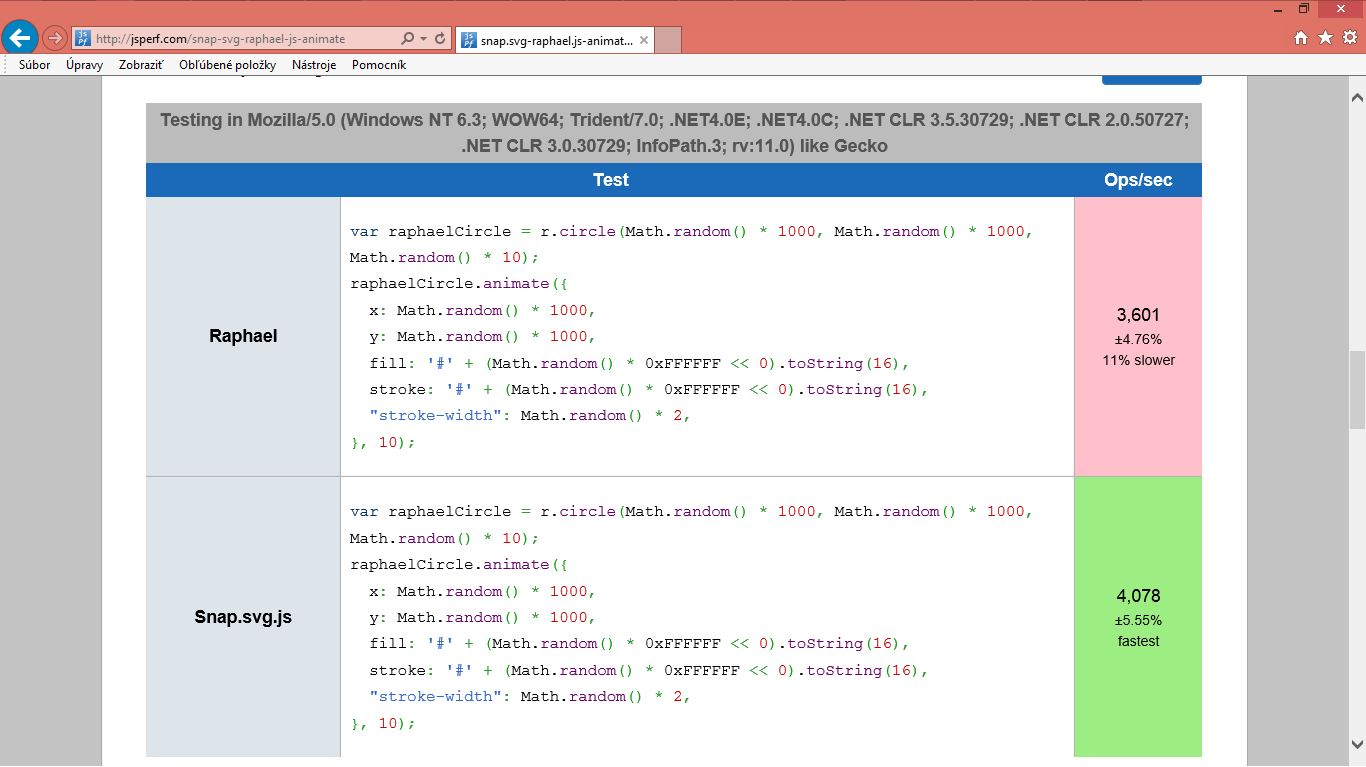
\includegraphics[width=0.7\linewidth]{obrazky/testovanieSnapVsRaphael2.jpg}
\caption{Po spustení testovania výkonnosti knižníc Raphael.js vs Snap.svg.js - výsledky pre konkrétny prehliadač}
\label{fig:vyslMozila}
\end{figure}

Výsledky testu sú nasledovné: 
\begin{itemize}
\item pre mobilné zariadenia a ich príslušné webové prehliadače sú v tabuľke \ref{tab:mobily}
\item pre súčastné a staršie verzie webových prehliadačoch, ktoré sú spustiteľné na počítačoch sú v tabuľke \ref{tab:pocitace}
\item pre staršie verzie webových prehliadačoch sú v tabuľke %\ref{tab:starsie}
\end{itemize}



\begin{table}[H]
	
\begin{center}

\begin{tabular}{|l|c|c|}
	\hline \textbf{Webový prehliadač} & \textbf{Raphael.js (ops/sec)} & \textbf{Snap.svg.js (ops/sec)} \\ 
	\hline Android 4.1.2 & 292 & 292 \\ 
	\hline Chrome 11.0.6996 & 1 283 & 1 283 \\ 
	\hline Chrome Mobile 42.0.2311 & 181 & 266 \\ 
	\hline Firefox Mobile 33.0 & 285 & 414 \\ 
	\hline 
\end{tabular} 
\end{center}

\caption{Výsledky testu pre mobilné zariadenia}
\label{tab:mobily}
	\end{table}

\begin{table}[H]
\begin{center}
		\begin{tabular}{|l|c|c|}
		\hline \textbf{Webový prehliadač} & \textbf{Raphael.js (ops/sec)} & \textbf{Snap.svg.js (ops/sec)} \\ 
		\hline Chrome 42.0.2311 & 2 753 & 2 171 \\ 
		\hline Epiphany 3.10.3 & 2 609 & 2 609 \\ 
		\hline Firefox 37.0. & 3 626 & 3 626 \\ 
	
			\hline IE 10.0 & 4 688 & 4 593 \\ 
			\hline IE 11 & 4 771 & 4 565 \\ 
			\hline Opera 25.0.1614 & 1 627 & 1 627 \\ 
			\hline Opera 29.0.1795 & 2 626 & 2 352 \\ 
			\hline Safari 5.1.7 & 3 249 & 3 050 \\ 
			\hline Iné & 1 432 & 1 427 \\ 
			\hline 
	
	\end{tabular} 
	
\end{center}
	\caption{Výsledky testu pre deskopové zariadenia}
	\label{tab:pocitace}
\end{table}

Súhrný graf výsledkov webových prehliadačov je na obrázku \ref{fig:graf}. Aritmetický priemer pre knižnicu Raphael.js je 2263.230769 a pre Snap.svg.js je 2175. Najlepšie výsledky dosiahol Internet Explorer verzia 11. 

 \begin{figure}[H]
\centering
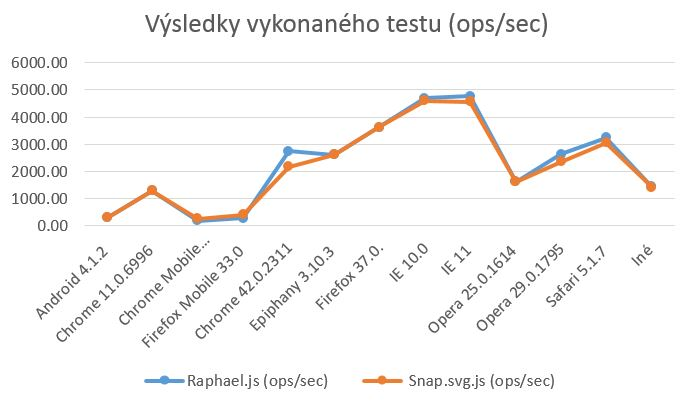
\includegraphics[width=0.9\linewidth]{obrazky/graf.JPG}
\caption{Graf výsledkov pre webové prehliadače}
\label{fig:graf}
\end{figure}



\section{Raphael.js vs Snap.SVG.js vs SVG.js - attr()}
Tento test bol zameraný na porovnanie výkonosti troch knižníc, ktoré umožňujú animáciu SVG. V teste sa vytváralo hmomadne kruhy s náhodnými hodnotami a následne po vykonaní iterácie sa vymazali. Iterácií prebehlo 100. 
%http://jsperf.com/raphael-vs-snapsvg-attr/7

multiple circles moved to the back

Kód testu: 

\begin{lstlisting}[language = html]
<script src="jquery.min.js"></script>
<script src="snap.svg.js"></script>
<script src="raphael.js"></script>
<script src="svg.js"></script>

<div id="raphael"></div>
<svg id="snap"></svg>
<svg id="svgjs"></svg>

<script>
var ncircs = 100;
var circs;

removecircs = function () {
    for (var i=0; i<circs.length; i++) {
      circs[i].remove();     }
   circs=[];};

var r = Raphael('raphael', 800, 600);
rapcirc = function () {
  var raphaelCircle = r.circle(400, 300, 150);
  raphaelCircle.attr({
    cx: raphaelCircle.attr('cx') + Math.random() * 50 - 25,
    cy: raphaelCircle.attr('cy') + Math.random() * 50 - 25
  }).toBack();
  circs.push(raphaelCircle);
  if (circs.length>=ncircs) removecircs();
};

var s = Snap('#snap');
s.width=800;
s.height=600;
snapcirc = function () {
  var snapCircle = s.circle(400, 300, 150);
  snapCircle.attr({
    cx: snapCircle.attr('cx') + Math.random() * 50 - 25,
    cy: snapCircle.attr('cy') + Math.random() * 50 - 25
  }).prependTo(s);
  circs.push(snapCircle);
  if (circs.length>=ncircs) removecircs();
};


var draw = SVG('svgjs').size(800, 600);
svgcirc = function () {
  var svgjsCircle = draw.circle(300).center(400, 300);
  svgjsCircle.attr({
    cx: svgjsCircle.attr('cx') + Math.random() * 50 - 25,
    cy: svgjsCircle.attr('cy') + Math.random() * 50 - 25
  }).back();
  circs.push(svgjsCircle);
  if (circs.length>=ncircs) removecircs();
};
</script>
 
\end{lstlisting}

Výsledok testu pre webový prehliadač je na obrázku~\ref{fig:graf2}

 \begin{figure}[H]
\centering
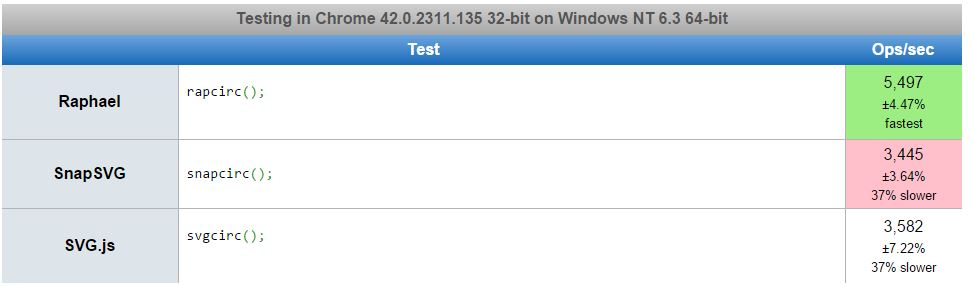
\includegraphics[width=0.7\linewidth]{obrazky/test2.JPG}
\caption{Test pre funkciu attr() pre webový prehliadač Chrome 42}
\label{fig:graf2}
\end{figure}





Výsledky vykonaných testov vo viacerých webových prehliadačoch sú na obrázku \ref{fig:graf3}.

 \begin{figure}[H]
\centering
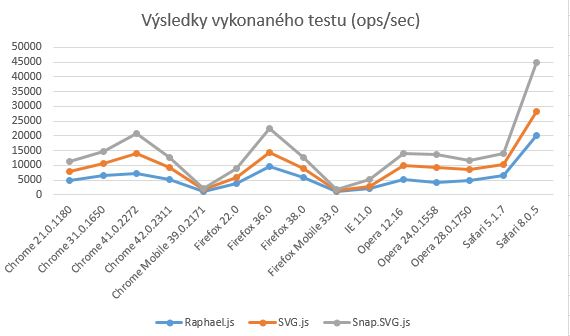
\includegraphics[width=0.9\linewidth]{obrazky/graf3.JPG}
\caption{Graf výsledkov pre webové prehliadače}
\label{fig:graf3}
\end{figure}


\begin{table}[H] \begin{center} \begin{tabular}{|l|c|c|c|} \hline \textbf{Webový prehliadač} & \textbf{Raphael.js} & \textbf{SVG.js} & \textbf{Snap.SVG.js}  \\ \hline Chrome 21.0.1180 & 4875 & 3147 & 3164  \\ \hline Chrome 41.0.2272 & 7268 & 6866 & 6589  \\ \hline Chrome 42.0.2311 & 5261 & 3976 & 3427  \\ \hline Chrome Mobile 39.0.2171 & 1073 & 746 & 398  \\ \hline Firefox 22.0 & 3946 & 1856 & 3158 \\ \hline Firefox 38.0 & 5835 & 2965 & 3783 \\ \hline Firefox Mobile 33.0 & 1156 & 309 & 426 \\ \hline IE 11.0 & 2272 & 724 & 2208 \\ \hline Opera 12.16  & 5239 & 4645 & 4092 \\ \hline Opera 24.0.1558 & 4150 & 5134 & 4461\\ \hline Opera 28.0.1750 & 4830 & 3827 & 3154 \\ \hline Safari 5.1.7 & 6709 & 3475 & 3919\\ \hline Safari 8.0.5 & 20226 & 8084 & 16438 \\ \hline \end{tabular} 
	
\end{center}
	\caption{Výsledky testu pre viaceré webové prehliadače (ops/sec)}
	\label{tab:test3}
\end{table}




\clearpage






\section{SVG vs Canvas}
%Počet objektov SVG 
%Zložitosť SVG - výpočtový výkon





%Sometimes there are outside influences that require a choice of technology that is, or is mostly, independent of functionality. For the question of using Canvas or SVG, there are two primary differentiators. Sometimes developer knowledge, skill set, and existing assets play a significant role into the choice of technologies. If a developer has deep knowledge of low level graphic APIs and limited knowledge of web technologies, the likely technology to choose is canvas.Also, performance is absolutely critical on high traffic websites. It is necessary to compare the performance characteristics of the two technologies. This might require the development of accessibility, custom styling, and more granular user interactions that do not come with canvas. It does not mean that canvas, though typically viewed as highly performant, is the obvious choice. The following graphs show the difference between of rendering time between SVG and Canvas objects.

Na obrázku \ref{fig:podpora23} sú zobrazené dva grafy, ktoré porovnavajú vlastnosti Canvas a SVG. 


Všeobecne platí, ak sa veľkosť obrazovky zvýši, plátno sa začne zmenšovať až na toľko pixelov, koľko je potrebné vykresliť. Pri SVG je to tak, ak sa počet objektov na obrazovke zvýši, tak začne neustále dané objekty pridávať do DOM.Tieto merania nie sú nevyhnutné presné a môžu sa zmeniť v závislosti od implementácie a platformy, hardvérovej akcelerácie grafiky. \cite{microsoft}


 \begin{figure}[H]
\centering
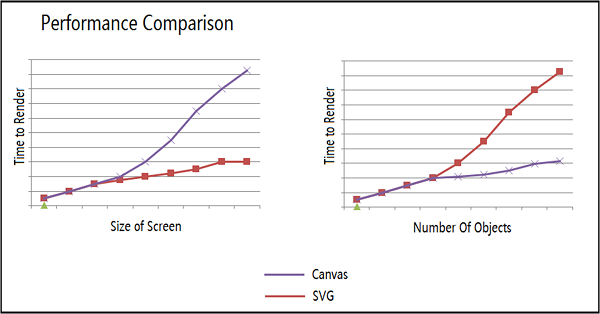
\includegraphics[width=1\linewidth]{obrazky/porovnanie}
\caption{Porovnanie výkonnosti Canvas vs. SVG}
\label{fig:podpora23}
\end{figure}






%Pre meranie výkonnosti vizualizácie grafických komponentov v reálnom čase zadefinujem v nasledujúce kritéria \begin{itemize}	\item počet komponentov, 	\item čas načítania stránky, 	\item čas vykonania zmeny atribútov v komponentoch.\end{itemize}Testy boli vykonané vo webovom prehliadači Chrome verzia 45 a Firefox verzia 40.  V teste boli použité nasledujúce navrhnuté komponenty:\begin{itemize}	\item teplomer, 	\item prečerpávacia stanica, 	\item trojcestný ventil, 	\item mapa Slovenska, 	\item prepravný pás. \end{itemize}Objekty boli v rovnakom zastúpení v jednom HTML súbore  v počtoch: 1,5,10,25, 50, 100.Ukážka testovacej situácie je na obrázku TODO SCREEN. A výsledky sú uvedené v tabuľke TODO TABULKA. \newpage Alebo vytvorim test -\url{http://jsperf.com/}- kde porovnam SVG smil animaciu s snap.svg.jsktore je v kapitole 4 - strana vtedy bola 20

%
%\url{http://www.sitepoint.com/advanced-snap-svg/}
%Performance Improvements
%
%One way to improve performance when manipulating the DOM is using DocumentFragments. Fragments are minimal containers for DOM nodes. Introduced a few years ago, they allow you to inexpensively manipulate entire subtrees, and then clone and add a whole subtree with n nodes to our page with 2 method calls instead of n. The actual difference is explained in details on John Resig’s blog.
%
%Snap allows for native use of fragments as well, with two methods:
%
%Snap.parse(svg) takes a single argument, a string with SVG code, parses it and returns a fragment that can be later appended to any drawing surface.
%
%Snap.fragment(varargs) takes a variable number of elements or strings, and creates a single fragment containing all the elements provided.
%
%Especially for large svg drawings, fragments can lead to a huge performance saving, when used appropriately.
%
%
%\newpage
%
%%http://www.html5rocks.com/en/tutorials/speed/high-performance-animations/
%
%\url{http://caniuse.com/#feat=svg-html}
%
%
%***********************
%
%Animácia pozície 
%- transform: translate(npx, npy);
%
%Animácia škály 
%- transform: scale(n);
%
%Animácia otáčania
%- transform: rotate(ndeg)
%
%Animácia neprehľadnosti 
%- opacity: 0..1;
%
%*************************
%
%%\url{http://www.svgopen.org/2008/papers/74-HighPerformance_GML_to_SVG_Transformation_for_the_Visual_Presentation_of_Geographic_Data_in_WebBased_Mapping_Systems/}
%
%
%\textbf{Transformation}
%\textit{scale}(sx, sy) - zmenim veľkosť tvaru na danane suradnice, 
%\textit{translate}(tx, ty) - presuniem na ine miesto - zmenim suradnice 
%
%%\url{https://developers.google.com/web/fundamentals/performance/rendering/optimize-javascript-execution?hl=en}
%
%Podpora svg v prehliadačoch
%\url{http://caniuse.com/#feat=svg}
%
%\url{http://www.schepers.cc/svg/blendups/embedding.html}
\chapter{Vzorová sada}

Vzorová sada grafických komponentov SCADA systémov obsahuje:
\begin{itemize}
	\item Thermometer,
	\item Triple Valve, 
	\item Map of Slovakia,
	\item Pumping station, 
	\item Conveyor belt 
	
\end{itemize}

\begin{figure}[H]
\centering
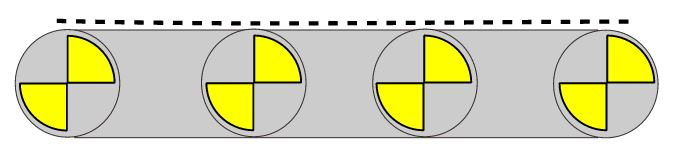
\includegraphics[width=0.7\linewidth]{obrazky/belt}
\caption{}
\label{fig:belt}
\end{figure}


\begin{figure}[H]
	\centering
	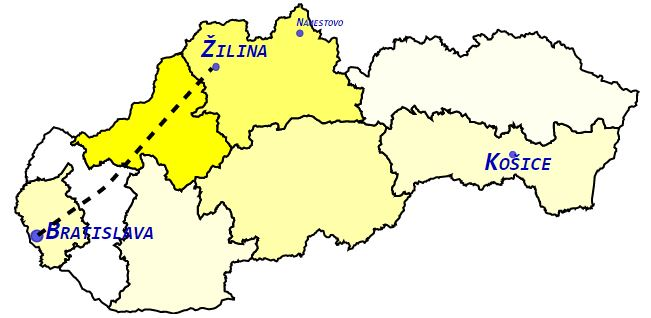
\includegraphics[width=0.7\linewidth]{obrazky/map}
\caption{}
\label{fig:map}
\end{figure}
\begin{figure}[H]
	\centering
	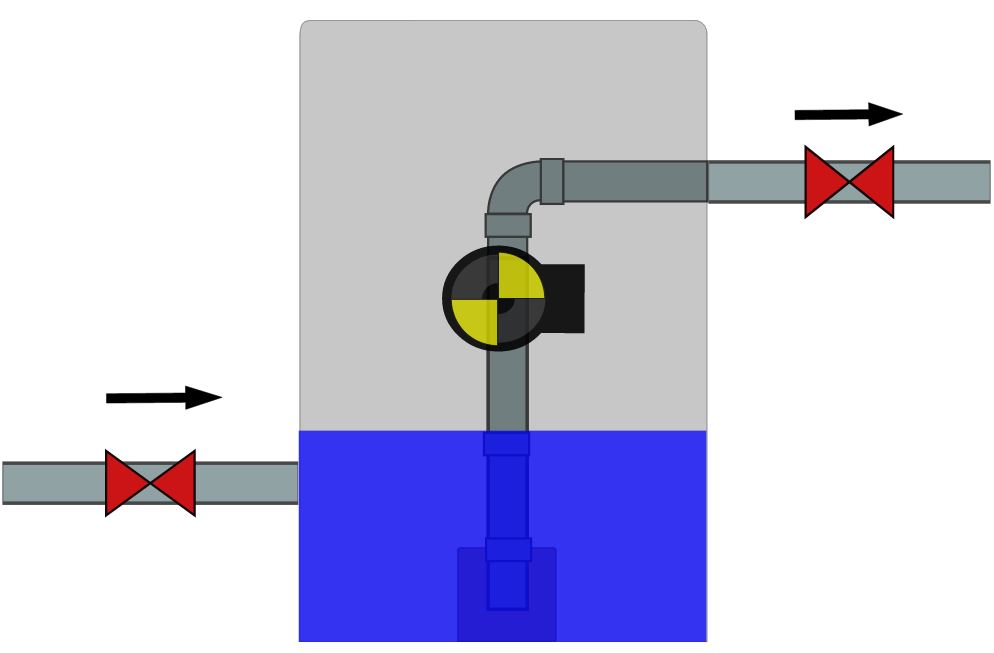
\includegraphics[width=0.7\linewidth]{obrazky/pump}
\caption{}
\label{fig:pump}
\end{figure}
\begin{figure}[H]
	\centering
	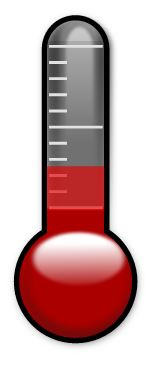
\includegraphics{obrazky/thermometer}
\caption{}
\label{fig:thermometer}
\end{figure}

\begin{figure}[H]
\centering
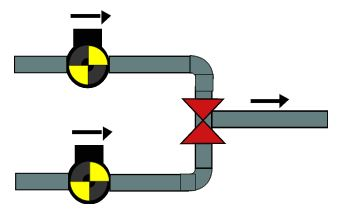
\includegraphics[width=0.7\linewidth]{obrazky/trippleValve}
\caption{}
\label{fig:trippleValve}
\end{figure}

\chapter*{Záver}

Cieľom práce bolo navrhnúť riešenie pre vizualizáciu SCADA komponentov vo webovom prehľadači. Mojou úlohou bolo i to, vytvoriť univerzálnejší postup pre animáciu komponentov.  Doterajšie riešenie bolo nepraktické, nebolo to modulárne a vyžadovalo to  zásah do riadiacej časti animácie. Navrhnuté riešenie odstraňuje použitím HTML5 štandardou - SVG, JavaScript. 

Cez Inkscape sa nakreslí komponent, a cez JavaScript pomocou knižnice Snap.svg.js sa manipuluje. Podarilo sa mi aj to, aby bol výsledný prvok responzívny aj na iných platformách ako napríklad tablety. SVG podporujú všetky moderné webové prehliadače.

Moje riešenie používa knižnicu a softvér, ktorý je open-source. Všetky zdrojové kódy práce sú v Git repository na GitHube.






%%%%%%%%%%%%%%%%%%%%%%%%%%%%%%%%%%%%%%%%%%%%%%%%%%%%%%%%%%%%%%%%%%%%%%%%%%%%%
\begin{thebibliography}{99}                               
	 \label{literatura}
%\addcontentsline{toc}{section}{Literatúra}
%\addcontentsline{toc}{chapter}{Zoznam použitej literatúry}




\bibitem{Dawber}
Dawber D.,
{\it Learning Raphael JS Vector Graphics }, 
 Packt Publishing, 2013, ISBN 978-1-78216-916-1
         
 
 
\bibitem{Wilson} Wilson CH., {\it RaphaelJs Graphic and visualization on the web} , 
O'Reilly Media, 2013, ISBN 978-1-449-36536-3
         

\bibitem{Haverbeke}
Haverbeke M., 
{\it Eloquent Javascript} 2. vyd. No Starch Press, 2014, ISBN 978-1-59327-584-6


\bibitem{Zakas}
Zakas N. Z., 
{\it JavaScript pro webové vývojáře Programujeme profesionálně},
 v1. vyd. Brno:Computer Press, a.s., 2009,  ISBN 978-80-251-2509-0

\bibitem{Suehring}
Suehring S., 
{\it JavaScript krok za krokem},
1. vyd. Brno:Computer Press, 2008, ISBN 978-80-251-2241-9

\bibitem{ZakasA}
Zakas N. C., McPeak J., Fawcett J.,
{\it Profesionálně Ajax},
Zoner Press, 2007,  ISBN 978-80-86815-77-0

\bibitem{Eisenberg}
Eisenberg D. J., {\it SVG Essentials}, 
O'Reilly Media 2002, ISBN  978-0-596-00223-7,  dostupné na \url{http://commons.oreilly.com/wiki/index.php/SVG_Essentials}

\bibitem{Richardson}
Richardson L., Amundsen M., {\it RESTful Web APIs} 
1. vyd. O'Reilly Media, 2013, 
ISBN 978-1-449-35806-8

\bibitem{Allamaraju}
Allamaraju S., {\it RESTful Web Services Cookbook} 
1. vyd. O'Reilly Media, 2010, 
ISBN 978-0-596-80168-7

\bibitem{snapsvg}
The JavaScript SVG library for the modern web,
\url{http://snapsvg.io/}.


\bibitem{Raphael}
\url{ http://raphaeljs.com/}

\bibitem {d3js}
\url {http://d3js.org/}

%\bibitem{snapsvg}
% \url{http://snapsvg.io/}
 
 \bibitem{svgjs}
 \url{http://www.svgjs.com/}


\bibitem {Inkscape}
Inkscape is a professional vector graphics editor for Windows, Mac OS X and Linux. It's free and open source.
\url {http://www.inkscape.org/en/about/features/}

\end{thebibliography}	%  Literatura
%%%%% \MakeBibliography 

\chapter*{Zoznam skratiek}
\begin{acronym}
\acro{API}{Application Programming Interface}
\acro{CSS}{Cascading Style Sheets}
\acro{D3}{Data Driven Document}
\acro{DOM}{Document Object Model}
\acro{DPI}{Dots Per Inch}
\acro{GIF}{Graphics Interchange Format}
\acro{HTML}{Hyper Text Markup Language} 
\acro{JPEG}{Join Photographic Experts Group} 
\acro{JSON}{JavaScript Object Notation}
\acro{PPI}{Pixels Per Inch}
\acro{REST}{Representational State Transfer}
\acro{RGB}{Red Green Blue}
\acro{RPC}{Remote Procedure Call}
\acro{SCADA}{Supervisory Control and Data Acquisition} 
\acro{SMIL}{Synchronized Multimedia Integration Language}
\acro{SVG}{Scalable Vector Graphics} 
\acro{VML}{Vector Markup Language}
\acro{W3C}{World Wide Web Consortium}
\acro{WYSIWYG}{What You See Is What You Get}
\acro{XML}{EXtensible Markup Language}
\acro{MES} {Manufacturing Execution System}
\acro{RAD} {Rapid Application Development}
 
\end{acronym}

%pridat typy licencie.. 



\appendix
\chapter{UML diagramy}
	\section{Usecase diagram použitia SCADA systémov}
	\begin{figure}[H]
		\centering
		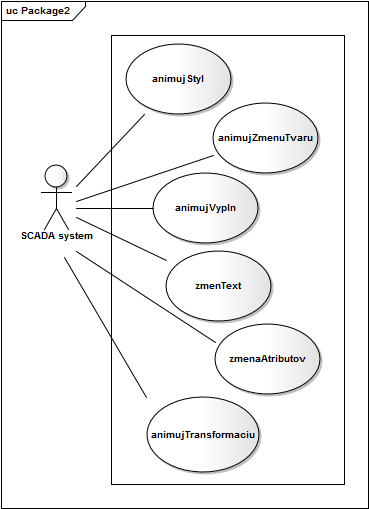
\includegraphics[width=0.50\linewidth]{uml/usecase.png}
		\caption{Usecase diagram použitia SCADA systémov}
		\label{fig:USECASE}
	\end{figure}

	\section{Postup načítania SVG súboru v HTML}
\begin{figure}[H]
	\centering
	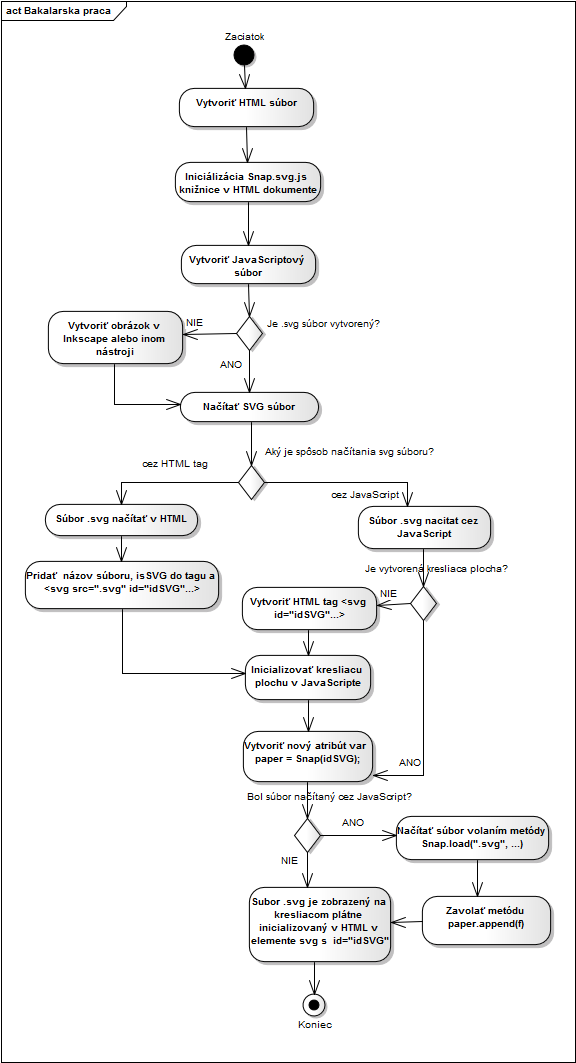
\includegraphics[width=0.70\linewidth]{uml/aktivityInicializacie}
	\caption{Postup načítania SVG súboru v HTML dokumente}
	\label{fig:aktivity1}
\end{figure}

\section{Postup zistenia id elementu}

\begin{figure}[H]
	\centering
	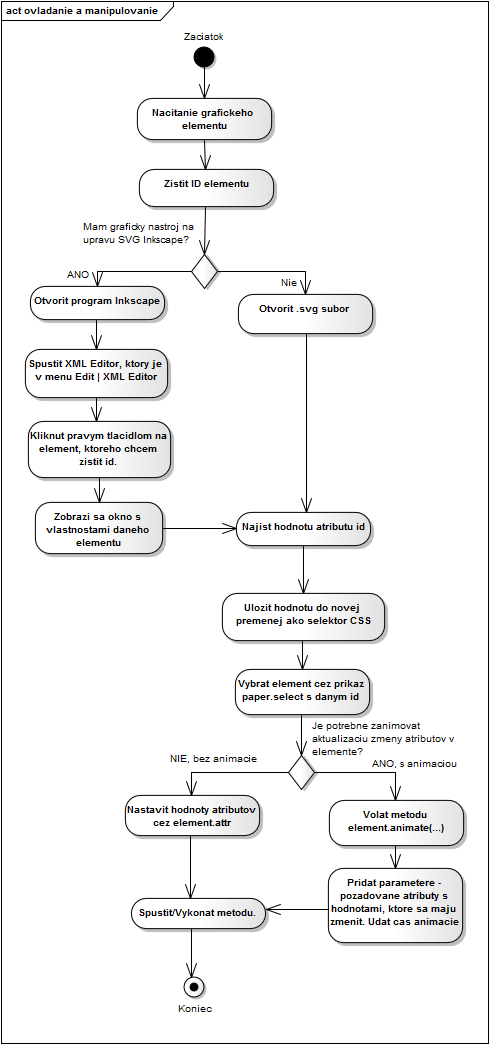
\includegraphics[width=0.6\linewidth]{uml/aktivity2.png}
	\caption{Postup zistenia id elementu a jeho aktualizovanie}
	\label{fig:ovladanie}
\end{figure}







\section{Diagram tried vzorovej sady}
Diagram tried vzorovej sady je na obrázku \ref{fig:classD} . 
\begin{figure}[hp]
	\centering
	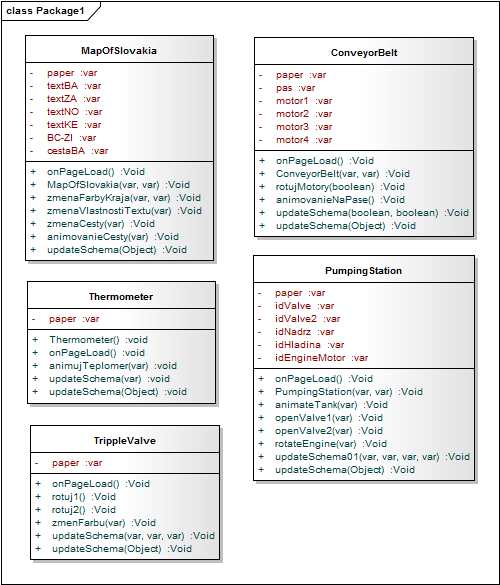
\includegraphics[width=0.9\linewidth]{uml/classDiagramTried}
	\caption{Diagram tried vzorovej sady grafických komponetov}
	\label{fig:classD}
\end{figure}





\end{document}